\documentclass[12pt]{book}
\usepackage{graphicx}
\usepackage[a4paper,inner=36mm,outer=18mm,top=30mm,]{geometry}
%\usepackage[doublespacing]{setspace} 
\usepackage{bm}
\usepackage{siunitx}
\usepackage{titling}
\usepackage{tabularx}
\usepackage{hyphenat}
\usepackage{amsmath,amsfonts,amssymb,amsthm,mathtools}
\usepackage{hyperref}
\usepackage{algpseudocode}
\usepackage{algorithm}
\usepackage{bbm}
\usepackage{caption}
\usepackage{subcaption}
\usepackage{multirow}
\usepackage{gensymb}
\usepackage{calc}
\usepackage{tabto}
\usepackage{natbib}

\DeclareMathOperator*{\argmin}{argmin}
\DeclareMathOperator*{\argmax}{argmax}

\setcitestyle{authoryear, open={(},close={)}}

\begin{document}

\title{Thesis}
\author{Emilio Dorigatti}

\maketitle


\section*{Acknowledgments}
todo

\newpage

\section*{Summary}
todo

\tableofcontents

\listoffigures

\listoftables

\chapter{Introduction}

\section{Problem}

Climatology, or climate science, studies the long-term average weather conditions. In the last few decades, climate scientists found evidence of ongoing changes in Earth's climate, most notably, a general increase in average temperature; in the long run, this and other changes can potentially have a devastating impact on life on our planet. Regardless of the causal effect of human activities on it, having a solid understanding of the climate allows us to find the best way to mitigate its change, and to preserve our planet.

Climate science is an extremely difficult field, for a number of reasons. First, climate is evident, by definition, only over long periods of time and large distances, making the usual scientific approach of testing hypotheses by conducting experiments inapplicable; instead, climate scientists have to rely on historical data. Second, the atmosphere is a complex and chaotic system, which must be described through systems of nonlinear differential equation. They can be used to create numerical simulations, and the resulting predictions compared to historical data to assess the accuracy of the theory. Furthermore, the chaotic character of the atmosphere makes it impossible to study parts of it in isolation from others, as small scale phenomena affect large scale ones, and vice versa. In spite of this, it is useful to split the atmosphere in vertical layers and horizontal zones, in order to differentiate among conditions and phenomena typically occurring in one area or the other.

The troposphere contains most of the air mass in the atmosphere, and occupies the lowest 10 to 12 kilometers of the atmosphere. This is where weather happens, and it can be divided in a number of sub-layers, the lowest of which is the \emph{atmospheric boundary layer}: it is the region of the atmosphere that is affected by the conditions of the surface. Most human activities happen in this layer, and it is responsible for a large part of the diffusion and transport of aerosol such as, among others, pollutants. Yet, the physics governing the atmospheric boundary layer is not fully understood, and the theory is lacking. One important issues in the study of the atmospheric boundary layer is the derivation of flux-profile relationships for wind and temperature: they essentially relate the transport of momentum and heat by the turbulence (flux) with the change of wind speed/temperature with altitude (profile). The state of the art relationships are defined by the Monin-Obukhov Similarity theory in terms of the instability parameter $\xi$, computed as the height above surface scaled by turbulence due to horizontal wind and vertical air movement due to variations in heat. Difficulties in measurements of relevant quantities make this theory accurate only up to 10-20\%, and applicable in a restricted set of conditions.

In stark contrast to the traditional, top-down approach of science, recent developments in information technology made bottom-up approaches possible. In this new way of thinking, existing data is used to automatically infer the "best" explanation for the measurements at hand, the underlying laws that originated that data. The field that makes this possible is called Machine Learning: it takes advantage of several methods coming from statistics, information theory, optimization theory, etc., to make computers learn from examples. Together with Natural Language Processing and Automated Planning, it is one of the three main branches of Artificial Intelligence, the sub-field of Computer Science that studies ways of making machines behave intelligently.

todo more fluff about ml ?

\section{Research Question}
Currently, limitations of the validity of the Monin-Obukhov similarity theory are not believed to be a likely explanation for the high scatter that is found in experimental studies, unless in highly stable conditions \citep{basicatm}. With the availability of micro-meteorological data from specialized observation sites such as Cabauw, in the Netherlands, and the recent developments in Machine Learning, this conjecture can be finally put to the test. More specifically, we pose the following \\

\textbf{Research Question 1:} Is it possible to use the data from the Cesar database to improve the Monin-Obukhov model of the flux-profile relationships, by using more predictors besides the instability parameter? \\

\textbf{Research Question 2:} (in case of an affirmative answer to the first research question): What impact do the different features have on the quality of the prediction? \\

Affirmative answers to these question would contribute to improve the quality of current global circulation models (large scale climate simulations). \cite{sheba} shows that, at least in difficult conditions, several simulation models produce flux estimates that are highly inaccurate, presenting low correlation (mostly below 0.3) and errors that are as large as the fluxes themselves. Since errors in the simulation accumulate over time, even slight improvements can greatly improve the accuracy of the results after years of simulated time. Improved flux-profile relationship can, therefore, yield more accurate estimates of the fluxes.

\section{Research Methodology}
todo

\section{Ethics and Sustainability}

reproducibility: using open data, following standards of reproducible research (open source and jupyter notebooks)

\section{Outline}
todo

\chapter{Background}
This chapter introduces the basic concepts the reader should be qualitatively familiar with, in order to understand the content of this thesis. It is assumed readers are already knowledgeable of simple mathematical concepts, such as calculus, linear algebra, statistics, and probability theory. Readers acquainted with the material should feel free to skip this chapter.

\section{Fluid Dynamics}
Fluid dynamics is the discipline that studies the flow of fluids; it has several branches that study different fluids, such as aerodynamics (the study of air motion) and hydrodynamics (the study of water motion). These disciplines are routinely applied when designing cars, airplanes, ships, pipelines, etc.

\subsection{Laminar and Turbulent flow}
There are two distinct ways in which particles in a fluid can move: laminar flow and turbulent flow. In the former, all the particles move orderly, perhaps with a different speed, but all in the same direction, whereas in the latter the movement of particles is highly chaotic and unpredictable, and tends to dive rise to eddies of varying sizes. People are most familiar with the distinction between the two through the smoke rising from a cigarette, which starts smooth and becomes turbulent shortly thereafter, as in figure \ref{fig:smoke}. The kind of flow in under specific conditions can be predicted using the Reynolds number $Re$, which is the ratio between inertia forces, favoring turbulent flow, and viscosity forces, stabilizing the fluid towards laminar motion:

$$
Re=\frac{\rho u L}{\mu}=\frac{uL}{\nu}
$$

With $\rho$ the density of the fluid, $u$ its velocity, $L$ a characteristic linear dimension of the system under consideration, $\mu$ and $\nu$ the kinematic and dynamic viscosity of the fluid. The viscosity describes, intuitively, how much the molecules of the fluid tend to stick together and resist motion by generating drag. For example, water has low viscosity, and honey has high viscosity.

Since turbulence is random, it is usually studied in terms of the statistical properties of physical quantities through the Reynolds decomposition; given a quantity $a(s,t)$ which varies in space and time, we can compute its average

$$
\overline{a}(s)=\frac{1}{T}\int_{T_0}^{T_0+T}a(s,t)dt
$$

and the deviation from the average

$$
a'(s,t)=a(s,t)-\overline{a}(s)
$$

By definition, $\overline{a'}=0$, which means that all the effects of turbulence are contained in $a'$. Common statistical properties such as variance and covariance are expressed respectively as $\overline{a'a'}$ and $\overline{a'b'}$.

\begin{figure}
\caption{Smoke from a cigarette, and the transition from laminar to turbulent flow.}
\label{fig:smoke}
\centering
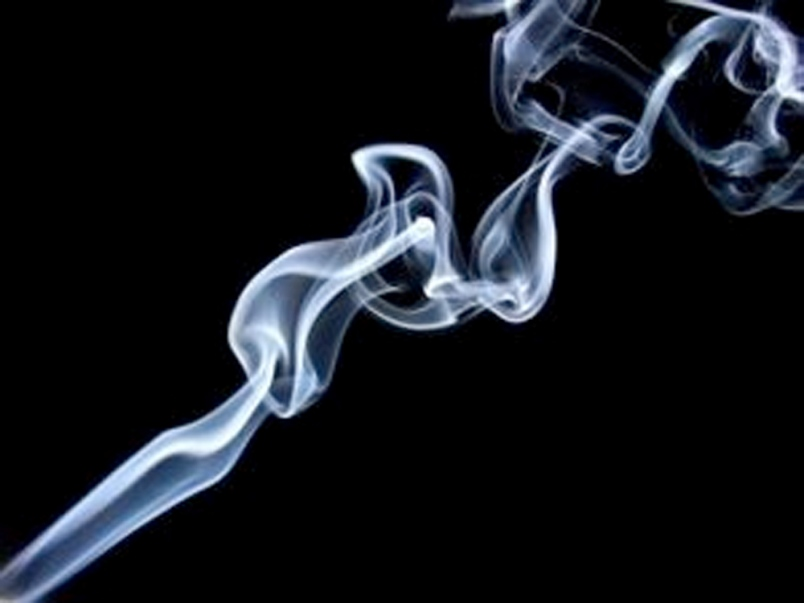
\includegraphics[width=0.5\textwidth]{images/smoke}
%https://www.google.se/search?client=ubuntu&q=cb+edits+smoke+png&tbm=isch&tbs=simg:CAQSlAEJkNL0D0I-7I0aiAELEKjU2AQaBAgVCAAMCxCwjKcIGl8KXQgDEiWoGUHnAegBsQw9sgxAlgawDIYnhSCHJ4okqzemIYgksCiVIKw3GjDJWGns8ZAx_17dvQFajhuRydFWdlJwDNo3VGI7iBUyNViewQZEJmiaYWGUhTUgxQOUgBAwLEI6u_1ggaCgoICAESBLt5JWoM&sa=X&ved=0ahUKEwiit7jKxKXZAhUBiCwKHTapCLQQ2A4IJygB&biw=1916&bih=948
\end{figure}


\subsection{The Boundary Layer}
In the context of fluid dynamics, the boundary layer is the region where a fluid flows close to a solid surface. Imagine a laminar flow close to a solid surface; because of viscosity, the molecules flowing near the surface move slower, and, in the limit, the velocity of the molecules in direct contact with the surface is 0 (this is called the \emph{non-slip condition}). Thus, the velocity of the fluid increases smoothly, continuously and monotonously with the distance from the solid, until it reaches the \emph{free-flow} velocity, after which it stays constant. The region close to the surface, where the fluid moves slower, is called the \emph{boundary layer}, and is the region where the viscosity of the fluid influences its motion. Its height $\delta$ can be defined when the local velocity surpasses a certain threshold, such as 99\% of the free-flow velocity.

\begin{figure}
\caption{Turbulent boundary layer at the edge of a canal; water flows from right to left.}
\label{fig:bl}
\centering
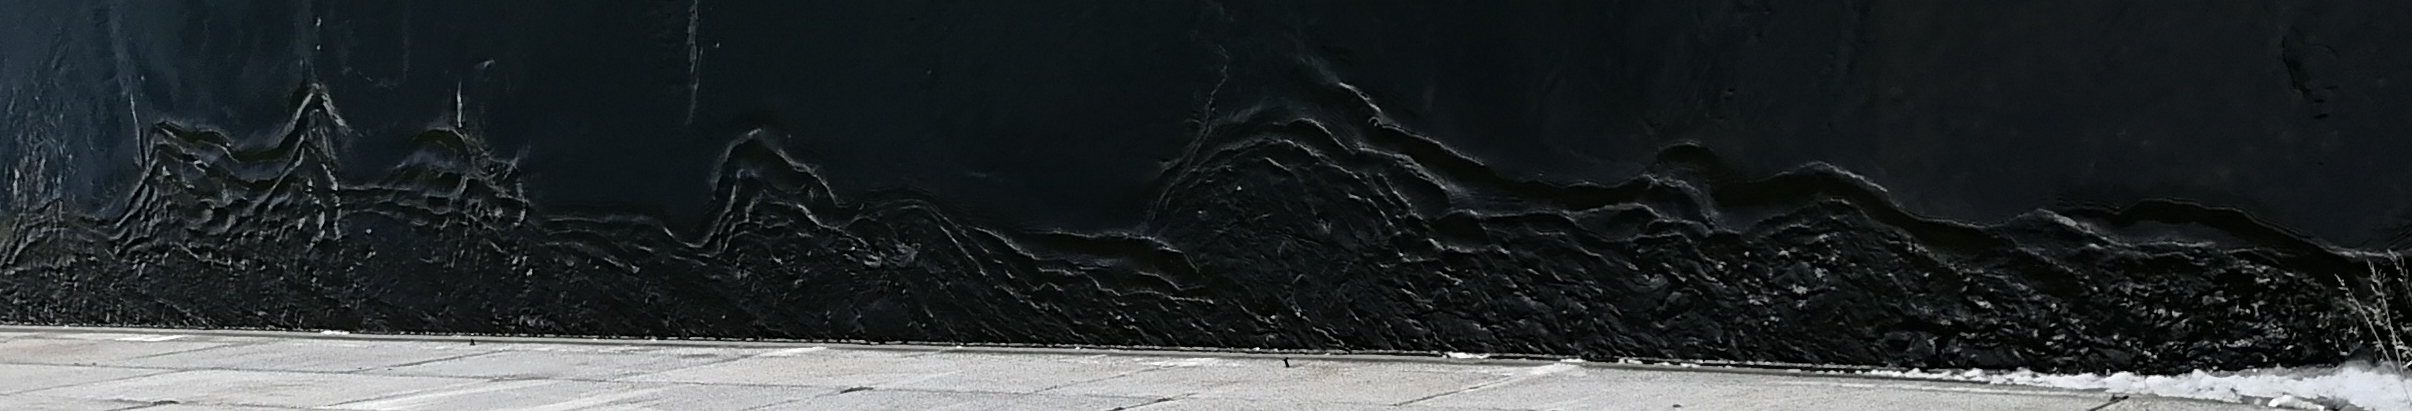
\includegraphics[width=\textwidth]{images/bl}
\end{figure}

The variation of velocity with distance from the surface, $\partial\overline{u}/\partial z$, is called \emph{shear}, and, together with viscosity, determines the materialization of turbulence in the flow. Every layer of fluid is squeezed between a faster moving layer above and a slower moving below; in high shear conditions, this causes high stress on the particles, and prevents them from moving orderly, thus leading to turbulent motion. Figure \ref{fig:bl} shows turbulence forming close to the wall in a canal, where the water flows from right to left. Viscosity and the no-slip condition prevent this phenomenon to arise in a region very close to the solid surface, called the \emph{laminar (or viscuous) sub-layer}, where we still find laminar motion.

The strength of the turbulence is proportional to $u_{rms}=(\overline{u'^2})^{1/2}$, which is, in turn, proportional to the shear. Again, because of the no-slip condition, $u_{rms}$ is zero at $z=0$, increases in the laminar sub-layer, and decreases to 0 at the end of the boundary layer, assuming laminar flow outside of it. Higher free-stream velocity generates higher shear, more turbulence, and a thinner laminar sub-layer. The strength of turbulence can be written in units of velocity, resulting in the \emph{friction velocity}, computed as $u_*=(\tau/\rho)^{1/2}=(\nu\cdot\partial\overline{u}/\partial z)^{1/2}$, where $\tau$ is the shear stress, $\rho$ is the density of the fluid, $\nu=\mu/\rho$ is the kinematic viscosity, and $\mu$ the dynamic viscosity. Therefore, the friction velocity increases with shear and viscosity, and decreases with density; it is proportional to the free-stream velocity and the turbulence strength, and inversely proportional to the height of the laminar sub-layer.

The mean velocity $\overline{u}$ increases linearly within the laminar sub-layer, then logarithmically until the end of the boundary layer, thus the shear decreases further away from the surface. In the logarithmic sub-layer, the velocity is computed as $\overline{u}(z)=u_*(\log z - \log z_0)/\kappa$, where $z_0$ is the characteristic roughness of the surface, and $\kappa$ is the von Karman's constant, whose value is around 0.4 [citation needed]. The characteristic roughness depends on the texture of the surface, and its relationship with the height $\delta_s$ of the laminar sub-layer; if the roughness scale is smaller than $\delta_s$, the logarithmic velocity profile is not affected by the texture, because the laminar sub-layer completely covers the variations on the surface, and we have the so-called smooth turbulent flow. If, on the contrary, the bumps in the surface are larger than $\delta_s$, the laminar sub-layer follow the profile of the surface, and the logarithmic velocity profile is altered depending on the texture, a regime called rough turbulent flow.

\section{The Atmospheric Boundary Layer}
The atmosphere is composed by air, which is behaves like fluid. Therefore, close to the Earth's surface, in the region called \emph{atmospheric boundary layer}, we find the same effects described in the previous section. Additionally, there are other phenomena that complicate things further, such as the temperature of the surface, which changes widely from day to night and from Summer to Winter, the rotation of the Earth, the varying roughness of the surface, due to cities and vegetation, etc. The effect of the surface on the first few hundred meters of the atmosphere is the main focus of \emph{boundary layer meteorology}. 

The height of the atmospheric boundary layer (hereafter abbreviated as ABL) typically varies between 100 and 1000 meters, highly depending on the conditions, and it is always turbulent. There are two main instabilities driving turbulence in the ABL:

\begin{itemize}
\item Shear instability: caused by shear, the mechanism described in the previous section. This happens at high Reynolds number, and, by using typical values for the ABL, we find $Re$ well above $10^6$.
\item Rayleigh-Bernard (also known as buoyancy driven) instability: is caused by the decrease of potential density\footnote{the potential density is the density that a parcel of air would attain if brought at a standard reference pressure adiabatically, i.e. disallowing exchanges of heat with its surroundings. Potential density is useful to compare densities irrespectively of pressure, i.e. altitude} with height, or, in other words, when warm fluid is below cold fluid; the warm fluid will rise, and the cold fluid will drop, a phenomenon called \emph{convection}. During hot Summer days, the surface is much warmer than the air, thus the air close to the surface will heat and tend to rise.
\end{itemize}

Turbulence has the very important role of transport and mix of air properties, such as heat, moisture, particles, aerosols, etc. This is especially true in \emph{unstable} conditions, when the air moving upwards (e.g. because it is warmer) is less dense than the air moving downwards; when the contrary happens, the ABL is called \emph{stable}.

The ABL can be divided in two main sub-layers: the inner surface layer and the outer Ekmann layer. This distinction is mainly done based on the scale of the dominating turbulent eddies: they are much smaller than the height of the ABL in the surface layer, and of comparable size in the outer layer.

It is very important to have a macroscopic understanding of the turbulent processes in the ABL, because they happen at length and time scales too small to be simulated in global climate models. The process of expressing the result of turbulence as a function of large scale parameters is called parametrization; having realistic models is essential in order to conduct precise simulations of the global climate in the scale of tens or hundreds of years, because errors tend to accumulate and amplificate as the simulation goes on. Other fields that benefit from the study of the ABL are urban meteorology (interested in the dispersion of pollutants), agricultural meteorology (interested in the formation of frost and dew, the temperature of the soil, etc.), aviation (predict fog and strong winds), and so on.

\subsection{Surface Fluxes}
A flux measures the amount of a physical quantity that flows through a surface. In the context of boundary layer meteorology, we are interested in the flows through the surface of earth, because, through them, the surface and the atmosphere exchange energy; these fluxes are thus measured in \si{\watt\per\square\meter}. The main source of energy for the surface is short-wave radiation coming from the sun, and long-wave radiation coming from the atmosphere and the clouds. A small amount of long-wave radiation is emitted from the surface, therefore let the net radiative flux be $R$, positive when the surface gains energy.

The main fluxes by which the surface gains or loses energy to the atmosphere are called the turbulent flux of \emph{sensible heat} $H$, also called kinematic heat flux, and the turbulent flux of \emph{latent heat} $\lambda E$, also called kinematic flux of water vapor/moisture. The difference between the two is that the former causes an actual change of temperature, whereas the latter does not affect temperature\footnote{imagine a pot of boiling water; selecting a higher temperature on the stove will not increase the temperature of water above \SI{100}{\celsius}, but will make it boil faster. The additional heat introduced in the system is dissipated through increased evaporation}. The main causes of sensible heat fluxes are conduction and convection, whereas the main cause of latent heat fluxes is water movement: condensation, evaporation, melting, etc. 

The final flux of interest is the soil heat flux $G$, which is the heat transferred into or out of the deeper layer of the soil and not given back to the atmosphere. These four fluxes are linked by the surface energy balance equation:

$$
R=H+\lambda E+G
$$

which states that the total incoming energy $R$ must be equal to the energy given back to the atmosphere $H+\lambda E$ (not counting long-wave radiation, which is accounted to in $R$) plus the energy absorbed by the surface $G$, assuming the temperature is constant. When the temperature is not constant, one can write a budget equation relating the changes in these quantities.

The turbulent fluxes $H$ and $\lambda E$ are constant in the surface layer. Experimentally, the energy balance is not always achieved \citep{cabauwinsitu} because of the difficulty in measuring fluxes due to eddy correlation being inaccurate.

\subsection{The Turbulence Kinetic Energy Budget}
Kinetic energy is energy stored in form of movement: faster or heavier objects have more kinetic energy than slower or lighter ones. The Reynolds decomposition allows us to decompose the kinetic energy of turbulent flows in two terms: one caused by the mean flow, and one caused by turbulence. This decomposition can be justified by examining the temporal spectrum of kinetic energy, shown in figure \ref{fig:tkespectrum}. Four peaks are visible, corresponding to different sources of kinetic energy: turbulence, day-night cycle, synoptic scale variability, lows and highs passing, and seasons. Importantly, there are few sources of kinetic energy in the 30 minutes to one hour time scale; this so-called spectral gap allows us to separate between turbulence and other sources of fluctuations in the atmosphere.

\begin{figure}
\caption{Long term average of atmospheric kinetic energy at different time-scales. The peaks in the scale of days and months and years are due to the day-night and Summer-Winter cycles, the peaks in the monthly scale are due to baroclinic instability in the mid-latitude westerlies, and the peaks at one minute are due to convection and atmospheric turbulence \citep{tkespectrumsrc,tkespectrumorig}}
\label{fig:tkespectrum}
\centering
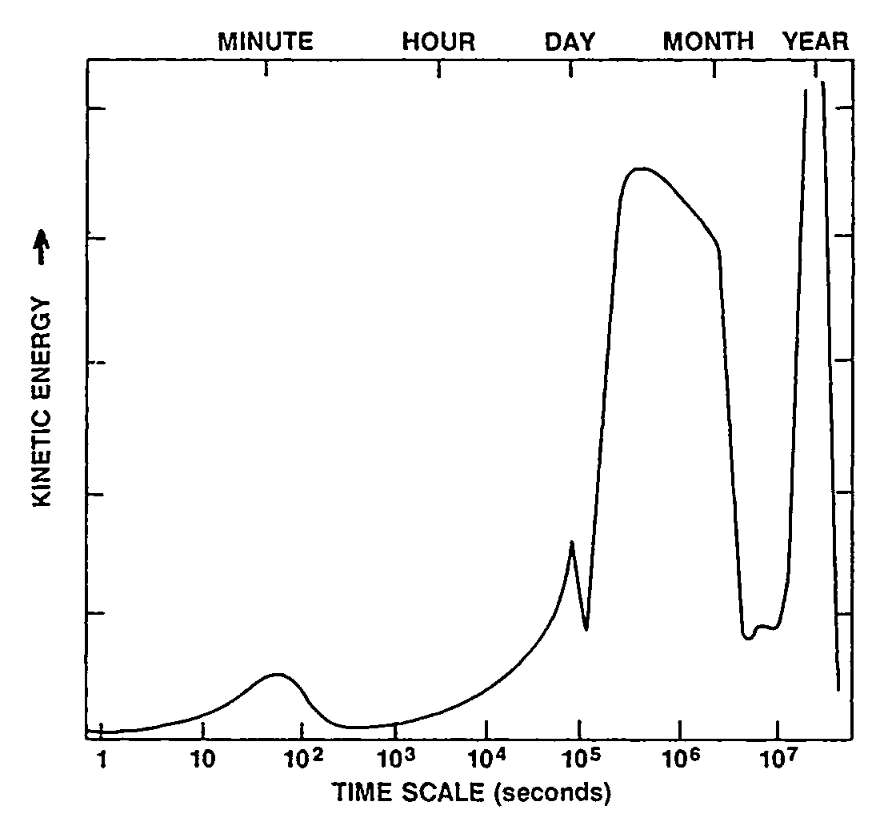
\includegraphics[width=0.5\textwidth]{images/kinetic_energy_spectrum}
\end{figure}

From now on, we will use a coordinate system with the $x$ axis aligned to the average horizontal wind direction, the $y$ axis perpendicular to it, and the $z$ axis pointing away from the surface. Then, we will use the letters $u$, $v$ and $w$ to denote the components of the wind along the axes $x$, $y$ and $z$ respectively; clearly, $\overline{v}=0$. Eddy fluxes can then be described in terms of covariances: let $\theta$ denote the potential temperature\footnote{the potential temperature is final temperature after bringing a parcel of air to a standard pressure adiabatically, i.e. not allowing exchange of temperature with the surroundings. It is a useful mean to compare temperatures irrespectively of pressure, i.e. altitude}, then $\overline{w'\theta'}$ is the turbulent heat flux, i.e. the sensible heat flux in the vertical due to turbulence. Usually the ABL  studied assuming homogeneous horizontal conditions, because they vary on a length scale larger than the height of the ABL. Because of this, the horizontal eddy correlations $\partial\overline{u'a'}/\partial x$ and $\partial\overline{v'a'}/\partial y$ are usually of negligible intensity, and are thus ignored. Note that this is not necessarily true when clouds are involved.

It is important to notice that turbulence is dissipative in nature. Consider a hot Summer day, where air is warmer close to the surface, and a circular eddy moving some air up and some down, so that the average motion is zero. The parcel of air moving up ($w'>0$) ends up being warmer than its surroundings ($\theta'>0$), while the one moving down ($w'<0$) will be colder ($\theta'<0$); the result is a net transport of heat through the eddy: $\overline{w'\theta'}>0$. On the contrary, imagine a cold night, where the air close to the surface is colder; the same eddy would transport a colder parcel of air upwards, and a warmer one downwards. In both cases, the end result would be a net transport of heat without transport of mass. Because of the ??? law, the eddy must lose energy, and thus dissipate over time.

Since turbulence changes over time, we are more interested in the change of kinetic energy, the \emph{turbulent kinetic energy budget}. A full derivation is out of the scope of this work, but its final form \citep{basicatm} can be derived from prime physical principles, resulting in

\begin{equation}
\frac{\partial\overline{{e'}^2}}{\partial t}
=\underbrace{\overline{u'w'}\frac{\partial\overline{u}}{\partial z}}_P
-\underbrace{\frac{g}{T}\overline{w'\theta'}}_B
+\underbrace{\frac{\partial}{\partial z}\frac{\overline{w'{e'}^2}}{2}}_{T_t}
+\underbrace{\frac{1}{\rho}\frac{\partial\overline{p'w'}}{\partial z}}_{T_p}
+\epsilon
\end{equation}

Where ${e'}^2={u'}^2+{v'}^2+{w'}^2$. The $P$ term is the production due to shear, $B$ is the production due to buoyancy, $T_t$ is the turbulent transport of TKE by large-scale eddies, $T_p$ is the transport due to pressure, and $\epsilon$ is molecular dissipation due to viscosity. $P$ and $B$ are the most prominent terms, and the transport terms are close to zero in neutral conditions \citep{basicatm}.

The $P$ term is always positive, as energy is taken from the mean flow to the turbulent one. On the other hand, the contribution from buoyancy can be either positive or negative, depending on the difference of temperature between a parcel of air moved by the turbulence and the surrounding air. When $\overline{w^\prime\theta^\prime}$ is negative, the turbulence is moving cold air upwards and warm air downwards; these parcels of air will try to undo the effect of turbulence, thereby increasing the overall kinetic energy. A similar reasoning goes for when the heat flux is positive.

\subsection{Monin-Obukhov Similarity Theory}
\label{sec:most}
One of the factors to distinguish laminar from turbulent flow is the length scale $L$ of the system. This length scale for the ABL was derived by A. M. Obukhov in 1946, and forms the basis of the similarity theory. According to this theory, the normalized wind and temperature profiles can be expressed as an unique function of $\xi=z/L$:

\begin{equation}
\label{eq:most_l}
L=-\frac{u_*^3}{\kappa\frac{g}{\theta_v}\frac{Q}{\rho c_\rho}}
=-\frac{u_*^3 T_v}{\kappa g \overline{w'\theta_v}}
\end{equation}

\begin{equation}
\label{eq:phi_m}
\frac{\partial\overline{u}}{\partial z}\frac{kz}{u_*}=\phi_m(\xi)
\end{equation}

\begin{equation}
\label{eq:phi_h}
\frac{\partial\overline{\theta_v}}{\partial z}\frac{kz}{T_*}=\phi_h(\xi)
\end{equation}

With

\begin{itemize}
\item $g=\SI{9.81}{\meter\per\square\second}$ the acceleration due to Earth's gravity
\item $\kappa=0.4$ the von Karman constant

\item $\theta_v$ virtual temperature\footnote{potential temperature of dry air if it had the same density as moist air. It allows to use formulas for dry air when the air is not dry.}, obtained as

\begin{equation}
\label{eq:vtemp}
\theta_v=\theta\frac{1+r_v/\epsilon}{1+r_v}=\theta(1+0.61\cdot q)
\end{equation}

Where $\theta$ is the air temperature, $r_v$ is the mixing ratio, $q=r_v/(1+r_v)$ the specific humidity, and $\epsilon$ is the ratio of the gas constants of dry air and water vapor, roughly 0.622.

\item $\rho$ the air density, computed from the pressure $P$ and the specific gas constant for dry air $R=\SI{287.058}{\joule\per\kilo\gram\kelvin}$ as

$$
\rho=\frac{P_0}{RT_v}
$$


\item $c_\rho$ specific heat of dry air, \SI{1005}{\joule\per\kilo\gram\per\kelvin} at \SI{300}{\kelvin}
\item $Q$ the buoyancy flux, approximated by $H+0.07\lambda E$ and measured in \si{\watt\per\square\meter}
\item $\overline{w'\theta_v}=Q/\rho c_\rho$ the flux of virtual potential temperature, measured in \si{\kelvin\meter\per\second}
\item $T_*=-\overline{w'\theta}/u_*$
\end{itemize}

The stability parameter $\xi$ is positive for stable conditions, where wind shear dominates the production of TKE, and negative for unstable conditions, where buoyancy is the main contributor to turbulence. It approaches 0 in the limit of neutral stratification (i.e. $\partial\overline{\theta}/\partial z=0$), because the temperature flux goes to 0 causing $L$ go to infinity.

todo talk about the method in \citep{cabauw_abl} to compute L

The universal functions $\phi_m$ and $\phi_h$ must be determined experimentally. This is no easy task, and considerable effort has been devoted to it; one of the greatest difficulties lies in obtaining accurate and unbiased measurements, especially the fluxes. \cite{hogstrom88} is a meta-study that aggregates and improves many previous results, and suggests the following expressions:

\begin{align}
\phi_m(\xi)&=\begin{cases}
\label{eq:phi_m_coeff}
\mathrlap{(1-19.3\xi)^{-1/4}} \hphantom{0.95(1-11.6\xi)^{-1/2}} & -2<\xi<0 \\
1+6\xi & 0<\xi<1\\
\end{cases} \\
\phi_h(\xi)&=\begin{cases}
0.95(1-11.6\xi)^{-1/2} & -2<\xi<0 \\
0.95+8\xi & 0<\xi<1
\end{cases}
\end{align}



The Monin-Obukhov similarity theory is only applicable in the surface layer, at heights much larger than the aerodynamic roughness length, and with $\vert\xi\vert<2$; when $\vert\xi\vert$ is too large, the eddies do not feel the effect of the surface anymore. Even under ideal conditions, the predictions of this theory are accurate up to 10-20\% [foken 2006].

\section{Machine Learning}
The goal of Machine learning is to develop algorithms that allow computers to learn from examples. Learning is intended as the ability of inferring general rules from the available examples, so that new, previously unseen examples can be correctly characterized. The set of samples from which the computer is supposed to learn is called the \emph{training set}, and each sample is a sequence of numbers describing its attributes, or \emph{features}. There are three approaches in machine learning:

\begin{itemize}
\item \emph{Supervised} learning: in this setting, the examples are composed of an input and a desired output, and the goal is to build a model that can correctly predict the output given the input. There are different algorithms depending on the type of output: \emph{regression} algorithms predict continuous output, while \emph{classification} algorithms predict discrete output.

\item \emph{Unsupervised} learning: in this setting, no output is available. The task of the algorithm is to figure out hidden relationships between the samples in the training set, for example whether they form clusters, or there are anomalous samples, or the correlation between features of the examples.

\item \emph{Reinforcement} learning: in this setting, the computer is free to act in an environment and to observe how the environment responds to its actions. Additionally, it receives a \emph{reward} for every action it takes, and the goal of the computer is to learn a sequence of actions that maximizes the received reward. Reinforcement learning is often applied in robotics [citation] and game playing [alphazero citation].
\end{itemize}

A supervised machine learning model uses a set of parameters to compute the output value starting from the input features. The actual parameters values are learned from the training set in a process called \emph{training}. This process is controlled by another set of parameters called hyper-parameters, whose value can be found from the training data as well. Whereas the parameters control the relationship between input and output, hyper-parameters control the "character" of the learning algorithm, such as how eager or conservative it is in learning minute details in the features. Learning too many details can be detrimental, because some differences can be due to noise, rather than actual differences.

The next sections describe the theory of learning, a general technique to estimate the parameters of a regression model, and introduce several machine learning algorithms for regression.

\paragraph{Notation:} Scalars are denoted in \textit{italic}, vectors (always column) and matrices in \textbf{bold}. The training set contains $N$ training samples, indexed by $n$, and each sample is a pair of feature vector $\bm x_n\in\mathbb{R}^D$ and a target value $t_n\in\mathbb{R}$. The feature vectors are grouped in the $N\times D$ matrix $\bm X=\left[\bm x_1\dotsb\bm x_N\right]^\intercal$ and the target values in the $N\times 1$ vector $\bm t=\left[t_1,\ldots,t_n\right]^\intercal$. Models are parametrized by a parameter vector $\bm\theta$ and their output for the feature vector $\bm x_n$ is $f_n=f(\bm x_n;\bm\theta)$. The vector containing both parameters and hyper-parameters is denoted with $\bm\Theta$.

\subsection{Learning Theory}
The goal of supervised learning is to use the training examples $D=(\bm X, \bm t)$, independent and identically distributed according to an unknown distribution $p_{XT}$, to find a good prediction rule $\hat{f}:\mathcal{X}\rightarrow\mathcal{Y}$ among a family of available functions $\mathcal{F}$. In most practical cases, $\mathcal{X}=\mathbb{R}^D$ and $\mathcal{Y}$ is either $\mathbb{R}$ for regression or a subset of $\mathbb{N}$ for classification. The goodness of a prediction rule $f$ is measured through a \emph{loss function} $\ell:\mathcal{Y}\times\mathcal{Y}\rightarrow\mathbb{R}$ that tells, given a target value $t$ and a guess $y=f(x)$, how much the guess is off. The \emph{risk} of an estimator $f$ is simply its expected loss:

\begin{equation}
R(f)=\mathbb{E}_{(x,t)\sim p_{XT}}\left[\ell(f(x),t) \vert f \right]
\end{equation}

The ideal situation is to find the estimator $f^*$ that has the lowest risk; unfortunately this is not possible, because the distribution $p_{XT}$ is unknown. Since the training data is a sample from this distribution, we can compute the \emph{empirical risk} of $f$ on this set of examples instead:

\begin{equation}
\hat{R}(f)=\mathbb{E}_{(x,t)\sim D}\left[\ell(f(x),t)\vert f\right]=\frac{1}{N}\sum_{n=1}^N \ell(f(x_n),t_n)
\end{equation}

We can now use the empirical risk as a surrogate for the true risk, selecting the estimator

\begin{equation}
\hat{f}=\argmin_{f\in\mathcal{F}}\hat{R}(f)
\end{equation}

as our best guess. This procedure is called \emph{empirical risk minimization}. Note that $\hat{f}$ is a random function, because it depends on $D$, which is a random variable. An interesting question to ask is how good $\hat{f}$ actually is, or, in other words, what is its expected true risk $\mathbb{E}[R(\hat{f})]$ and how it compares to the lowest attainable risk $R(f^*)$. This latter quantity can be decomposed as

\begin{equation}
\mathbb{E}[R(\hat{f})]-R(f^*)=
\left(\mathbb{E}[R(\hat{f})]-\inf_{f\in\mathcal{F}} R(f)\right)
+\left(\inf_{f\in\mathcal{F}} R(f)-R(f^*)\right)
\end{equation}

Where the first term is the \emph{estimation} error incurred by not selecting the best possible estimator in $\mathcal{F}$, and the second term is the \emph{approximation} error caused by searching a good estimator in $\mathcal{F}$. They usually have opposite behavior:

\begin{itemize}
\item the estimation error is high when $\mathcal{F}$ is too complex for the data at hand, where complexity refers to the range of phenomena that can be accurately modeled by these functions. In other words, $\mathcal{F}$ contains many valid explanations that are equally good on the training set (they have low empirical risk $\hat{R}$), but are not accurate models of the underlying phenomenon $p_{XT}$, i.e. they do not generalize well (they have high risk $R$);
\item the approximation error is high when $\mathcal{F}$ cannot adequately model the phenomenon that we are trying to describe, i.e. when it does not contain any good explanation for it.
\end{itemize}

This decomposition is often referred to as the \emph{bias-variance decomposition}, where bias and variance refer to, respectively, approximation and estimation error.

The fundamental problem is to find a class of functions that is powerful enough to model $p_{XT}$, but not too powerful so as to contain too many good explanations, because we would not be able to choose. Equivalently, we want to find a good model, one that can explain the data we have, and generalize to new examples. This problem is known as \emph{model selection}, and is important to distinguish between model selection for \emph{identification}, and model selection for \emph{estimation}. In the former case, the goal is to obtain a model and its parameters, to be used on new prediction problems, whereas the goal of the latter is to obtain a realistic estimate of the performance that can be obtained on new data. This problem can be approached in two ways: by directly estimating approximation and estimation errors using hold-out sets, or by penalizing complex models in order to favor simpler explanations, even though they might have slightly higher empirical risk. The next sections describe these two approaches.


\subsection{Cross Validation}
\label{sec:cv}
The idea behind hold-out methods is to partition the available data in two smaller sets $D_T$ and $D_V$, usually of size 2/3 and 1/3 of the total, and use the \emph{training} set $D_T$ to choose $\hat{f}$ and $D_V$ to estimate its risk. Since $D$ is assumed to be a representative sample from $p_{XT}$, if the two partitions contain independent and identically distributed samples, the empirical risk on the \emph{validation set} $D_V$ can give us a glimpse on the generalization power of $\hat{f}$. This is because the validation set contains new samples that were not used to choose $\hat{f}$, thus the empirical risk on this set is an unbiased estimate of the true risk of the discovered model. This allows us not only to be confident about the performance of the estimator on unseen data, but also to compare different estimators. The problem of a single hold-out set is the variance of its estimate of the risk, which depends on the size of the validation set. This means that we are faced with a trade-off: use a lot of data to select a good estimator, but have high uncertainty in its estimated performance, or use less data and select a less powerful estimator, but have a more accurate picture of its performance.

The solution to this problem is to repeatedly perform this partitioning procedure so as to obtain many estimates of the risk, each on a different subset of validation samples, and average these results together. This can be done in a number of different ways:

\begin{itemize}
\item in random subsampling, the procedure above is simply repeated many times, by using two thirds random examples for training, and the remaining one third for validation;
\item In bootstrapping \citep{bootstrap}, the training set is created by taking $N=\vert D\vert$ examples \emph{with replacement} from $D$, and using the remaining examples for validation. This means that the validation set contains on average approximately 36.8\% of the samples in $D$, and the training set the remaining 63.2\%, with many duplicates;
\item In k-fold cross validation \citep{kfold}, $D$ is partitioned in $k$ subsets, and each of them is used in turn as validation set, while the others are used for training. This produces $k$ estimates of the true risk, coming from the $k$ subsets.
\end{itemize}

Regardless of the method used, the final estimate of the performance is the average of the estimates obtained from the individual trials. Every method has different properties regarding both the bias and the variance of the estimates, and there is considerable controversy on which method should be used in which situation. For example, \cite{cv_bootstrap} recommends using 10-fold cross validation for comparing models, because, although its estimate of the performance is biased, it has lower variance compared to bootstrapping; however, \cite{no_unbiased_cv} show that it is not possible to obtain an universal unbiased estimate of the variance of k-fold cross validation. \cite{cvmyths} further discusses this issue, and debunks some myths and commonly held misconceptions about cross validation, including the belief, consequent \cite{cv_bootstrap}, that 10-fold cross validation is always the best choice. Generally, there is a tradeoff in choosing the value of k, as high values yield estimates with lower bias, but higher variance \citep{cv_survey}, and are more computationally intensive.

todo nested cv \cite{nested_cv}

\subsection{Parameter Estimation for Regression}
\label{sec:regression_fit}

In this section, we describe a general framework, rooted in Bayesian statistics, for estimating the parameters of a regression model, while controlling overfitting. An advantage of Bayesian methods is that they offer a sound theoretical foundation for model selection, without requiring repeated experiments to choose among candidate models, although this mathematical rigor is not free from practical difficulties \citep{bayesian_model_selection, practical_bayesian_model_selection}.

A common assumption in the regression setting is that the observations are corrupted by additive Gaussian white noise, i.e. $t_n=y_n+\epsilon_n$, where $y_n$ is the "true" value, and $\epsilon_n\sim\mathcal{N}(0,\beta^{-1})$ is the noise. Let $f_n=f(\bm x_n;\bm{\theta})$ be the model's prediction for the sample $\bm x_n$, then we can write the probability of observing $t_n$, assuming that $f_n=y_n$, as:

\begin{equation}
\label{eq:model_pred_distrib}
p(t_n\vert \bm{x_n},\bm\Theta)=\mathcal{N}(t_n\vert f(\bm{x_n};\bm\theta),\beta^{-1})
\end{equation}

This probability is called \emph{likelihood} of the observation $t_n$, under the model $f(\cdot;\cdot)$ with parameters $\bm{\theta}$. Since the training data is assumed to be independent and identically distributed, the likelihood of the whole training set is

\begin{equation}
\label{eq:likelihood}
p(\bm{t}\vert\bm{X}, \bm\Theta)=\prod_{n=1}^N  \mathcal{N}(t_n\vert f(\bm{x_n};\bm\theta),\beta^{-1})
\end{equation}

And the predicted value $t$ for a new sample $\bm x$ is distributed as

\begin{equation}
p(t\vert \bm x, \bm X, \bm t)=\int
p(t\vert\bm x,\bm\Theta)\cdot p(\bm\Theta\vert \bm t, \bm X)\ \text{d}\bm\Theta 
\end{equation}

In practice, it is not feasible to compute this integral, and its value is dominated by the values of $\bm\theta$ close to the one that maximizes equation \ref{eq:likelihood} anyways; this is the gist of \emph{maximum likelihood estimation} (MLE). Note that, since the goal is to predict $y_n$, there is a high probability that the "true" parameters would \emph{not} be the ones with maximum likelihood. When a model learns the noise in the training data, it cannot generalize well to new, unseen data, because the noise is random. This situation is known as \emph{overfitting}, and tends to happen when the model is too complex relative to the amount of data available for training, and is related to high estimation error mentioned previously.

The risk of overfitting can be reduced with a number of \emph{regularization} strategies. A widely used strategy consists in including a prior distribution on the parameters of the model, and maximizing their posterior distribution, computed using Bayes theorem:


\begin{align}
\begin{split}
\label{eq:map}
p(\bm\Theta\vert\bm t, \bm X)&=\frac{p(\bm X, \bm t\vert\bm\Theta)\cdot p(\bm\Theta)}{p(\bm X, \bm t)}\\
&\propto p(\bm t\vert \bm X,\bm\Theta)\cdot p(\bm X\vert\bm\Theta)\cdot p(\bm\Theta)\\
&\propto p(\bm t\vert \bm X,\bm\Theta)\cdot p(\bm\Theta)
\end{split}
\end{align}


where we removed $p(\bm X,\bm t)$ and $p(\bm X\vert\bm\Theta)=p(\bm X)$ because they are constant for a given dataset, and we are not interested in the exact probability, but where it reaches its maximum value. This parameter estimation procedure is called \emph{maximum a posteriori} (MAP). Two commonly used prior distributions are the multivariate Laplace and the multivariate Normal, leading respectively to L1 and L2 regularization, when centered and symmetrical/spherical.

The maximization of the posterior can be done conveniently by maximizing its logarithm; this gives expressions that are easier to handle analytically, and give less numerical problems when computed. The MAP problem can be formulated as follows:

\begin{equation}
\bm\Theta^*=\argmax_{\bm\Theta}\ \log p(\bm t\vert\bm X,\bm\Theta)+\log p(\bm\Theta)
\end{equation}


If we assume a Gaussian likelihood like the one in equation \ref{eq:likelihood}, and a spherical Gaussian prior distribution $p(\bm\theta)=\mathcal{N}(\bm 0, \lambda\bm I)$, the MAP estimation of equation \ref{eq:map} becomes, after removing unnecessary constant terms,

\begin{equation}
\label{eq:least_squares}
\bm\theta^*=\argmin_{\bm\theta}\ L(\bm\theta)=\argmin_{\bm\theta}\sum_{n=1}^N\left( f(\bm x_n,\theta)-t_n\right)^2+\lambda\bm\theta^\intercal\bm\theta
\end{equation}

Where $L$ is the \emph{loss function}, in this case the sum-of-squares error. It is customary to use the mean squared error instead of the sum of squares because it results in smaller numbers and is readily interpreted; being only a constant factor away from \ref{eq:least_squares}, it does not transcend the essence of MAP estimation. The parameter $\beta$ can be estimated as well in a similar way, if necessary, and a fully Bayesian treatment allows to estimate $\lambda$, too. Depending on the model $f(\bm x_n,\bm\theta)$, \ref{eq:least_squares} can be solved analytically to yield a closed-form solution for $\bm\theta$.
 
When this is not possible, iterative optimization methods are employed. A widely used approach is called \emph{gradient descent}: the gradient of a function computed at a given location "points" to the steepest direction where the function's value increases. By repeatedly following the gradient, it is possible to reach a local maximum, and, in the opposite direction, a local minimum:

\begin{equation}
\bm\theta_{n+1}:=\bm\theta_n-\eta\cdot\nabla f(\bm x_n)
\end{equation}

the series $\bm\theta_1,\ldots,\bm\theta_n$ is guaranteed to converge to the local optimum at a rate of $O(n^{-1})$ if certain conditions are met \citep{gd_convergence}. \cite{numopt} describes more advanced optimization techniques that use the gradient and, possibly, the Hessian, such as Newton's. The gradient of $L(\bm\theta)$ is

\begin{equation}
\label{eq:least_squares_gradient}
\nabla_{\bm\theta}\log p(\bm\theta\vert\bm t,\bm X)
=2\sum_{n=1}^N \big(f(\bm x_n;\theta)-\bm t_n\big)\cdot\nabla_{\bm\theta}f(\bm x_n;\theta) + 2\lambda\bm\theta
\end{equation}

And its Hessian is

\begin{equation}
\label{eq:least_squares_hessian}
\nabla^2_{\bm\theta}\log p(\bm\theta\vert\bm t,\bm X)=2\sum_{n=1}^{N}\bigg[
\big(\nabla_{\bm\theta} f(\bm x_n;\bm\theta)\big)
\big(\nabla_{\bm\theta} f(\bm x_n;\bm\theta)\big)^\intercal
+\big(f(\bm x_n;\bm\theta)-t_n\big)\nabla^2_{\bm\theta}f(\bm x_n;\theta)\bigg]+2\lambda\bm I
\end{equation}

In some cases, the gradient and the Hessian can be approximated using a random subset of the training set, and, in extreme cases, a single sample. These variants are called \emph{minibatch} gradient descent and \emph{stochastic} gradient descent respectively. They both compute a noisy approximation to the true gradient, which can actually improve convergence and generalization of high-dimensional, non-convex loss functions such as those found in deep learning \citep{sgd_noise, bayesian_sgd}. Vanilla gradient descent can be greatly improved with a number of techniques, such as momentum \citep{gd_momentum}, adaptive learning rate \citep{adagrad, adadelta, adam}, and so on, see \cite{gd_overview} for an overview. 

\subsection{Hyper-parameter Optimization}
The previous section discussed some methods to find the best parameters for a model. In practice, though, finding good values for the hyper-parameters is often as important as fitting the model, since these hyper-parameters control the learning process itself.

A simple way to approach this problem is to choose some possible values for each hyper-parameter, try all the possible combinations, and pick the one that works best. Alternatively, one can sample each hyper-parameter from a probability distribution, and try many random combinations of values; \cite{random_search} showed that this latter method is surprisingly effective at this task, and scales much better than the former. Unfortunately, this procedure can overfit, too, so it has to be paired with some resampling technique such as cross validation. The procedure is simply to test every hyper-parameter combination on every fold, so that 50 combinations tested with 10-fold cross validation require to fit the model 500 times.

More sophisticated techniques treat hyper-parameter optimization as a regression problem, and use supervised machine learning to predict the performance of a given hyper-parameter combination, and to guide the search accordingly \citep{hyperopt}. Clearly, one should use models that are not sensitive to their own hyper-parameter setting, or the problem is just moved! For this reason, popular algorithms that are used for this are evolutionary algorithms and Bayesian non-parametric models.

\subsection{Ridge Regression}
\label{sec:ridge}
A linear regression model has the form $f(\bm x_n;\bm\theta)=\bm\theta^\intercal\bm x_n$; ridge regression is simply L2-regularized linear regression. This model is simple enough that the solution for equation \ref{eq:least_squares} can be found analytically in closed form:

\begin{equation}
\label{eq:ridge_solution}
\bm\theta^*=(\bm X^\intercal\bm X+\lambda\bm I)^{-1}\bm X^\intercal\bm t
\end{equation}

Notice that the term \emph{linear} in linear regression refers to linearity with respect to the parameters, not the features. In fact, new features can be added through the use of a possibly non-linear feature mapping $\phi:\mathbb{R}^D\rightarrow\mathbb{R}^M$, such that $\bm x^\prime_n=\phi(\bm x_n)^\intercal=\left[\phi_1(\bm x_n),\ldots,\phi_M(\bm x_n)\right]^\intercal$. Then, the model parameters can be fitted to the augmented training set $\bm\Phi=\bm X^\prime$, where $\bm\Phi$ is called the \emph{design matrix}. A typical feature added is a bias $\phi_1(\bm x)=1$.

\subsection{k-Nearest Neighbors}
The k-nearest neighbor model \cite{knn} predicts a value for a sample $\bm x$ by averaging the target values of the $K$ training samples that are closest to $\bm x$, possibly weighted by distance or some other metric. Let $\bm t_{(1)},\ldots,\bm t_{(k)}$ be the target values of the $K$ training samples closest to $\bm x$ according to a distance metric $d:\mathbb{R}^D\rightarrow\mathbb{R}$, then we have

\begin{equation}
f(\bm x)=\sum_{k=1}^K w_{(k)}\cdot\bm t_{(k)}
\end{equation}


Note that the k-nearest neighbors algorithm does not have parameters, only hyper\hyp{}parameters: $K$ itself, the distance function, and the weighting scheme. Typical distance functions are the Manhattan distance $d(\bm u,\bm v)=\sum_{d=1}^D\vert u_d-v_d\vert$ and the squared Euclidean distance $d(\bm u,\bm v)=\sum_{d=1}^D(u_d-v_d)^2$, and typical weights are uniform $w_{(k)}=1/K$ and based on distance $w_{(k)}=d(\bm x,\bm x_{(k)})/\sum_{k^\prime=1}^K d(\bm x,\bm x_{(k^\prime)})$.

\subsection{Gradient Boosted Trees}
Gradient boosting \citep{gradientboosting} is a general method of combining several weak predictors in order to obtain a stronger one. The final prediction for a sample is obtained as a weighted average of the predictions of the individual models:

\begin{equation}
\label{eq:gboost}
f_M(\bm x)=\sum_{m=1}^M \beta_m h(\bm x;\bm\theta_m)
\end{equation}

Each model $h_m$ and its weight $\beta_m$ are found by improving the predictions of $f_{m-1}$:

\begin{equation}
\label{eq:gboostjoint}
(\beta_m, \bm\theta_m)=\argmin_{\bm\theta,\beta}\sum_{n=1}^N L\left(
t_n, f_{m-1}(\bm x_n)+\beta h(\bm x_n,\bm\theta)
\right)
\end{equation}

Where $L$ is the loss function, such as the squared error introduced previously. This optimization problem can be challenging, depending on the specific form of $h_m$ and $L$. Actually, equation \ref{eq:gboostjoint} is equivalent to gradient descent in function space\footnote{meaning that you actually modify the function itself, not its parameters, as we did in section \ref{sec:regression_fit}. This provided that the parametric function $h$ is able to represent the gradient} \citep{boostinggd,greedyboosting}. This gradient can be computed explicitly on the $N$ training points, but we do not know how to compute it on the other points that are not in the training set\footnote{this is the essence of gradient descent in function space, since a function is defined for every point (at least the ones we consider in Machine Learning)}. The fundamental idea is to find a model that can predict this gradient, by training it on the dataset. This model is exactly $h$ with parameters $\bm\theta_m$:

\begin{equation}
\label{eq:gbtheta}
\bm\theta_m=\argmin_{\bm\theta}\sum_{n=1}^N \left[
-g_m(\bm x_n)-h(\bm x_n,\bm\theta)
\right]^2
\end{equation}

With $g_m$ being the gradient of $L$ with respect to $f_{m-1}$:

\begin{equation}
\label{eq:gbgrad}
g_m(\bm x_n)=\frac{\partial L(t_n,f_{m-1}(\bm x_n))}{\partial f_{m-1}(\bm x_n)}
\end{equation}

Then, the step size $\beta_m$ is obtained by line search, i.e. minimizing the loss function in the direction of the gradient:

\begin{equation}
\label{eq:gbbeta}
\beta_m=\argmin_{\beta}\sum_{n=1}^N L(t_n, \beta h(\bm x_n,\theta_m))
\end{equation}

This is now a tractable problem, since \ref{eq:gbgrad} can be computed easily, and both \ref{eq:gbtheta} and \ref{eq:gbbeta} are simple regression problems.

If $L(y_n,t_n)=(y_n-t_n)^2/2$, we have that $-g_m(\bm x_n)=f_{m-1}(\bm x_n)-t_n$, or, in other words, we are creating a new model by counteracting the errors of the current model! Other popular loss functions are the least absolute deviation, $L(y_n,t_n)=\vert y_n-t_n\vert$, in which case $-g_m=sign(t_n-f_{m-1}(\bm x_n))$, and the Huber loss:

\begin{equation}
\label{eq:huberloss}
L_\delta(t_n,y_n)=\begin{cases}
\frac{1}{2}(y_n-t_n)^2 & \vert y_n-t_n \vert \leq \delta \\
\delta(\vert y_n-t_n\vert-\frac{1}{2}\delta) & \vert y_n-t_n \vert > \delta \\
\end{cases}
\end{equation}

Which is robust to outliers as least absolute deviation, but does not penalize small errors too much, like least squares. WIn this case,

\begin{equation}
-g_m(\bm x_n)=\begin{cases}
t_n-y_n & \vert t_n-y_n\vert\leq\delta \\
\delta\cdot sign(t_n-y_n) & \vert t_n-y_n\vert>\delta
\end{cases}
\end{equation}

In summary, the gradient boosting algorithm starts with a simple prediction $f_0$, such as the average of the true values, builds a model of the form in equation \ref{eq:gboost} by iteratively applying equations \ref{eq:gbtheta} and \ref{eq:gbbeta}.

A popular choice is to use decision trees for $h$. Often, an additional \emph{learning rate} parameter is introduced to shrink the $\beta$ coefficients. Other hyper-parameters for this algorithm are $M$, the the number of boosting steps to perform, the number of examples to use to compute equations \ref{eq:gbtheta} and \ref{eq:gbbeta}, the number of features used to build the trees, their maximum depth, and so on.

A popular extension to vanilla gradient boosting is \emph{extreme gradient boosting} \citep{xgboost}, which essentially adds regularization to the loss function, helping to reduce overfitting, and provides better scalability.

\subsection{Gaussian Processes}
A Gaussian Process (GP) is a collection of an infinite number of random variables, such that the joint distribution of any finite subset of them is Gaussian. Intuitively, this allows us to define a distribution over functions, since there is a random variable for every point of the input space. We can sample a function out of a GP by obtaining the random variables at the points of interest; their distribution is a (multivariate) Gaussian, with a certain mean and covariance, and a sample from this distribution contains the values of the sampled function at the points we queried. This process is expressed as follows:

\begin{equation}
\label{eq:gp_marg}
p(\bm y\vert\bm X)=\int p(\bm y\vert \bm f)p(\bm f\vert\bm X)\text{d}f
\end{equation}

Where $\bm X$ are the query points, $\bm f$ a function sampled from the GP, and $\bm y$ the values of the function. By definition of GP, all the distributions in equation \ref{eq:gp_marg} are Gaussian, since the Gaussian distribution is self-conjugate. A GP is just a way of computing the mean and covariance of $\bm f$ given $\bm X$, i.e. $p(\bm f\vert\bm X)$; $\bm f$ is then a multivariate Gaussian, which we can manipulate as usual.

Consider the setting of ridge regression described in section \ref{sec:ridge}, where $\bm y=f(\bm X;\bm\theta)=\bm\Phi\bm\theta$, with $\bm\Phi$ being the design matrix. Recall that in section \ref{sec:regression_fit} we introduced the Maximum A Posteriori estimation method by using a prior distribution on the model parameters $\bm\theta$; this makes $\bm y$ a random variable itself. If we use an isotropic Gaussian for $\bm\theta$, we have that the distribution of $\bm y$ is again Gaussian with mean

\begin{equation}
\mathbb{E}[\bm y]=\mathbb{E}[\bm\Phi\bm\theta]=\bm\Phi\mathbb{E}[\bm\theta]=\bm 0
\end{equation}

and covariance

\begin{equation}
\text{cov}[\bm y]=\mathbb{E}[\bm y\bm y^\intercal]
=\bm\Phi^\intercal\mathbb{E}[\bm\theta^\intercal\bm\theta]\bm\Phi
=\alpha^{-1}\bm\Phi^\intercal\bm\Phi=\bm K
\end{equation}

Where $\alpha$ is the precision of the prior on $\bm\theta$. This is a simple GP with zero mean, and whose covariance between any two points can be computed as the dot product of their features.

In general, we can use any function $k$ to compute the covariance between two input points, as long as the resulting matrix $\bm K$, with $K_{ij}=k(\bm x_i,\bm x_j)$ is symmetric and positive semi-definite\footnote{this means that $\bm K^\intercal=\bm K$ and $\bm v^\intercal\bm K\bm v\geq 0$ for any $\bm X$ (used to compute $\bm K$) and $\bm v$. This condition is necessary for $\bm K$ to be a valid covariance matrix}. We call any such function  \emph{kernel}, a function $k:\mathbb{R}^d\times\mathbb{R}^d\rightarrow\mathbb{R}$ that, intuitively, expresses the similarity of any two input vectors. Mercer's theorem guarantees that for every symmetric positive-definite kernel there exists a basis function $\phi$, such that the kernel corresponds to the dot product in the space generated by $\phi$. In practice, this means that we do not have to explicitly define $\phi$, and that we can even use basis functions that create an infinite dimensional space. Commonly used kernels are the radial basis function kernel:

\begin{equation}
k(\bm x, \bm x^\prime)=\exp\left(-\frac{\Vert\bm x-\bm x^\prime\Vert^2}{2\sigma^2}\right)
\end{equation}

where $\Vert\bm x-\bm x^\prime\Vert^2=\sum_d(\bm x_d-\bm x_d^\prime)^2$ is the squared Euclidean distance, and which incidentally corresponds to an infinite dimentional basis function, and the linear kernel:

\begin{equation}
k(\bm x, \bm x^\prime)=\sigma^2\bm x^\intercal\bm x^\prime
\end{equation}

Furthermore, certain operations on a kernel generate another valid kernel, and kernels can be combined in certain ways to produce a new kernel. For example, the product of a kernel with a positive constant is a valid kernel, the sum and product of two kernels are valid kernels, etc. Generally, a kernel can have parameters, which we denote, as usual, as $\bm\theta$.

In order to use a Gaussian Process for inference (in the regression setting), we need to compute the predictive distribution $p(\bm y\vert\bm X, \bm t, \bm X^*,\bm\theta) $, where $\bm X^*$ is the matrix containing the vectors for which we want to predict the value $\bm y$. We know that the predictive distribution is Gaussian, therefore its mean $\bm\mu_{\bm y}$ and covariance $\bm\Sigma_{\bm y}$ can be obtained relatively easily, resulting in:

\begin{equation}
\label{eq:gp_pred_mean}
\bm\mu_{\bm y}=K_{\bm\theta}(\bm X^*,\bm X) K_{\bm\theta}(\bm X,\bm X)^{-1}\bm t
\end{equation}

\begin{equation}
\bm\Sigma_{\bm y}=K_{\bm\theta}(\bm X^*,\bm X^*)-K_{\bm\theta}(\bm X^*,\bm X)^\intercal K_{\bm\theta}(\bm X, \bm X)^{-1}K_{\bm\theta}(\bm X,\bm X^*)
\end{equation}

Where $K_{\bm\theta}(\bm A,\bm B)$ is a matrix whose $(i,j)$ cell equals to $k(A_i,B_j;\bm\theta)$. From these formulas, note that in order to use GPs, one needs to remember the kernel matrix, of size $N^2$ and invert it, an operation which has a computational complexity of $O(N^3)$; this makes GPs, and any method based on kernels, hard to scale up.

Up until now, we assumed the kernel was fixed, and treated $\bm\theta$ as hyper-parameters. We could use one of the methods described in section \ref{sec:cv} to find their values, but the Bayesian framework that we used to derive GP allows us to find $\bm\theta$, too, by maximizing $\log p(\bm t\vert\bm X,\bm\theta)$\footnote{obtained as in equation \ref{eq:gp_marg}, usually called log-marginal-likelihood, since we marginalized $\bm f$} with respect to $\bm\theta$. This function often has many local maxima, and is usually optimized by means of gradient descent.

Finally, the derivative of a GP is itself a GP, whose mean is \citep{gp_diff}:

\begin{equation}
\label{eq:gp_gradient}
\frac{\partial\bm y}{\partial\bm X_*}=\frac{\partial K_{\bm\theta}(\bm X_*,\bm X)}{\partial\bm X_*}K_{\bm\theta}(\bm X,\bm X)^{-1}\bm t
\end{equation}

We invite the reader to refer to \cite[Chapter~6]{bishop} for an in-depth treatment of kernel methods, including Gaussian Processes.


\chapter{Method}
This chapter describes how the data is collected (section \ref{sec:data_collection}) and used to re-create the flux-profile relationships (section \ref{sec:profiles}), as well as their prediction based on the Monin-Obukhov similarity theory (section \ref{sec:most_fit}). Then, we describe the main contribution of this thesis, namely how their prediction can be improved using machine learning techniques (section \ref{sec:model_fit}). Finally, we describe how the evaluation is performed (section \ref{sec:perf_eval}), and explicitly state the necessary criteria for a successful answer to the research questions (section  \ref{sec:success}).

\section{Data Collection}
\label{sec:data_collection}
The Cabauw Experimental Site for Atmospheric Research\footnote{\url{http://www.cesar-database.nl/}} (Cesar) is a consortium formed by eight Dutch institutes and universities, which collaborate to operate and maintain an observatory for micro-meteorological conditions near the village of Cabauw, the Netherlands. The data collected characterizes the state of the atmosphere and the soil, and their interaction via radiation and surface fluxes.

The observatory is surrounded by fields and no urban agglomerations is present within 15 kilometers; the land is flat with changes of altitude within a few meters over 20 kilometers. The main mast is 213 meters high and offers measurement levels every 20 meters; at each level there are three booms of length 10 meters that allow observations unobstructed by the main mast. There are three additional smaller masts of height 10 and 20 meters located close to the main mast, in order to obtain undisturbed measurements at the lower levels, and facilities to perform soil and surface observations.

The main focus of this project is on wind and temperature profiles, and the turbulent fluxes of sensible and latent heat. Additional variables, such as temperature and humidity, are needed to compute quantities of interest, most importantly the Obukhov length, and as possible predictors for the universal functions. There is one measurement for each variable every ten minutes, and missing measurements are gap-filled with a number of techniques. The data collected is always visually validated by an operator, which marks suspect or invalid sections of data

The Cesar observatory provides full information regarding data collection\footnote{\url{http://projects.knmi.nl/cabauw/insitu/observations/documentation}}, see in particular \cite{cabauwinsitu}, what follows is a brief summary of the most relevant sections.

\begin{figure}
\caption{Sonic anemometer to measure wind and optical open-path sensor to measure humidity at the 180m level of the Cabauw mast.}
\label{fig:cabauw_180m_instruments}
\centering
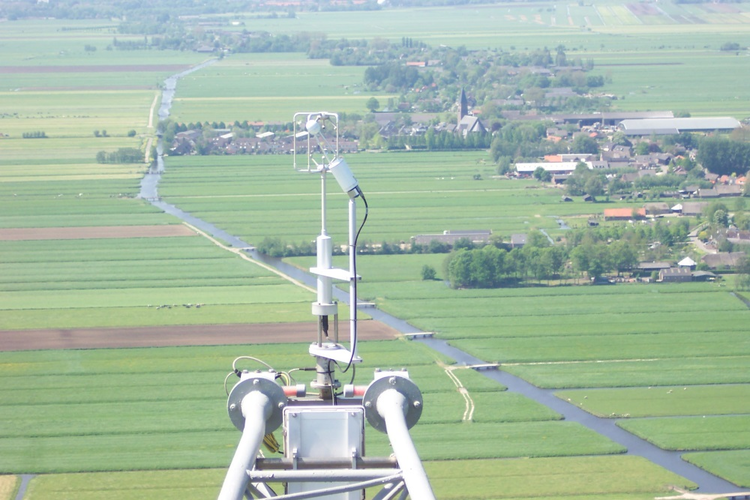
\includegraphics[width=0.75\textwidth]{images/cabauw_turbulence_instruments}
% https://www.knmi.nl/research/observations-data-technology/projects/cabauw-in-situ-measurements
\end{figure}

\subsection{Wind Speed Measurement}
Wind speed and direction are measured at heights of 200, 140, 80, 40, 20 and 10 meters, in either two or all three booms available. The wind vane that measures direction has a resolution of $1.5^\circ$, and the cup anemometer that measures wind speed has an accuracy of the largest between 1\% and \SI{0.1}{\meter\per\second}. \cite{windinstr} studied the threshold sensitivity of both instruments, and fount it lower than \SI{0.5}{\meter\per\second}, even though the measurements are inaccurate up to \SI{3}{\meter\per\second}.

For every ten minutes interval, the measurement comes from the instrument that is best exposed to the wind, and less affected by the obstruction caused by the mast. Corrections are then applied to the raw measurements to further attenuate the disturbance by the tower, following \cite{winddistortion}.

\subsection{Air Temperature and Dew Point Measurement}
Both air temperature and dew point are measured at heights of 200, 140, 80, 40, 20, 10 and 1.5 meters. The instruments at the highest four levels are located on the main tower, whereas 20 and 10 meters are measured in the smaller mast, and 1.5 meters is measured by the weather station. The resolution of the instruments is of \SI{0.1}{\celsius}, whereas the accuracy is \SI{0.1}{\celsius} for temperature and 3.5\% of relative humidity for the dew point (1.5\% after 2014). Low wind speed and high irradiation can result result in a few \SI{0.1}{\celsius} overestimate of the temperature \citep{tempoverestimate}, whereas the humidity can be over estimated when drying after dew, fog, or rain \citep{cabauwinsitu}.

\subsection{Net Radiation Measurement}
The Cabauw observatory measures both incoming and outgoing long- and short-wave radiation, and the net radiation is simply the combination of these four components. The basic operating principle of an instrument that measures radiation is to have a device coated with paint that is highly absorbing towards a certain range of frequencies; the temperature difference between the surface of this sensor and the body of the whole instrument generates an electrical potential that is proportional to the radiation absorbed by the sensor, after appropriate corrections.  The instruments that measure short-wave radiation are called \emph{pyranometers}, while long-wave radiation is measured by \emph{pyrgeometer}.  The instrument used to measure the net radiation has a pair or pyrgeometers, one facing up and one facing down, to measure the net long-wave radiation, and a pair of pyranometers arranged similarly to measure net short-wave radiation.

This instrument is positioned at \SI{1.5}{\meter} height, and is ventilated and heated to prevent formation of dew, that can make the measurements invalid.

\subsection{Soil Heat and $CO_2$ Flux}
todo


\subsection{Eddy Correlation}
\label{sec:eddy_correlation}
The eddy correlation technique is used to compute the turbulent surface fluxes of sensible and latent heat, as well as momentum and $CO_2$, starting from fluctuations in wind, temperature, and humidity.

These measurements are obtained with, respectively, a sonic anemometer, a sonic thermometer, and an optical open-path sensor. Sonic anemometers measure the wind speed by leveraging the fact that the speed of sound in free air is affected by the speed of the air itself; since the speed of sound is known, the wind speed can be easily recovered from the time a sound impulse takes to travel a short distance. By measuring the wind velocity along three orthogonal paths, the full wind vector can be recovered. Sonic thermometers work similarly, by leveraging the fact that the speed of sound is affected by the temperature of the medium it travels in. These instruments can take up to 100 measurements per second. Optical open-path sensors quantify the amount of water vapor and carbon dioxide in the air by emitting a ray of infrared light and measuring its intensity 10 to 20 centimeters further away. $H_2O$ and $CO_2$ molecules in the air absorb electromagnetic radiation at known frequencies, thus the concentration of water vapor and carbon dioxide can be inferred by measuring the attenuation at these wavelengths.

The eddy correlation technique measures fluxes by computing their sample covariance with the vertical wind speed. Let $w_t$ be the vertical wind speed at time $t$, then the turbulent vertical flux for the quantity $a$ is computed as follows:

$$
F_a=\frac{1}{T_2-T_1}\sum_{t=T_1}^{T_2}(w_t-\overline{w})(a_t-\overline{a})
$$

Where $\overline{w}$ and $\overline{a}$ are the averages of $w_t$ and $a_t$ for $T_1\leq t\leq T_2$. The fluxes in the Cesar database are computed every ten minutes, with 10 measurements per second.

The eddy correlation technique is far from perfect, see \cite{microhandbook} for a detailed summary of issues.

\subsection{Gap Filling}
\label{sec:gap_filling}
With gap-filling, missing measurements are replaced by synthetic values. The gap-filling method depends on the missing parameter and the duration of the period where data is not available. There are two classes of parameters: forcing parameters, which include wind, temperature, specific humidity, incoming radiation and rain, and validation parameters, which include the surface fluxes, outgoing radiation, and friction velocity.

For less than two hours of missing measurements, both forcing and evaluation parameters are gap-filled by interpolation of nearby values. For longer periods, forcing parameters are derived by transforming measures obtained from the nearby site of De Bilt, which are themselves gap-filled, if necessary. Evaluation parameters are computed with a vegetation model that uses the forcing parameters as input. The gap-filling procedure is performed by the Cesar consortium.


\subsection{Data Filtering}
\label{sec:data_filter}
Following other works in this field, such as \cite{boulder} and \cite{hogstrom88}, we exclude all the records where any of the following conditions applies:

\begin{itemize}
\item The sensible heat flux $H$ is smaller than \SI{10}{\watt\per\square\meter};
\item The friction velocity $u_*$ is smaller than \SI{0.1}{\meter\per\second};
\item The wind speed $\overline{u}$ is lower than \SI{1}{\meter\per\second}.
\end{itemize}

todo also mention dew point, soil heat (and that missing values are not imputed), net radiation, rain

\section{Flux-Profile Relationships}
\label{sec:profiles}

Since the turbulent fluxes and the friction velocity are measured at the surface level, we can compute the flux-profile relationships only at 10, 20 and 40 meters, because these quantities can be assumed constant only within the surface layer. It is very hard to know the exact height of the surface layer, because it depends on the weather and no exact formulas are known, but it is usually assumed to be 10\% as high as the boundary layer. Based on the typical height of the boundary layer, the surface layer is often higher than 40 meters and lower than 80. \cite{cabauw_z0} indeed reports that a large number of observations from Cabauw at \SI{20}{\meter} are inside the surface layer, the \SI{100}{\meter} level is already outside of the surface layer, and \cite{boulder} used the observations at \SI{50}{\meter} in their analysis, but not those at \SI{100}{\meter}.

todo http://bibliotheek.knmi.nl/knmipubTR/TR303.pdf says 60m is outside of the surface layer only in the morning, and 100m / 180m are inside later in the day

\subsection{Obukhov Length}

The Obukhov length is computed as in equation \ref{eq:most_l}, reported here:

$$
L=-\frac{u_*^3}{\kappa\frac{g}{\theta_v}\frac{Q}{\rho c_\rho}}
=-\frac{u_*^3 T_v}{\kappa g \overline{w'\theta_v}}
$$

The flux of virtual potential temperature can be computed following the formulas in section \ref{sec:most}, as the data contains all the necessary quantities; $u_*$ is given, as well as the specific humidity and the pressure. The Obukhov length is computed at each height level using the corresponding air temperature measurement, and the fluxes measured at the surface.


\subsection{Gradients}
\label{sec:gradients}
The flux-profile relationships are listed in equations \ref{eq:phi_m} and \ref{eq:phi_h}, and are reported here for the reader's convenience:

$$
\phi_m(\xi)=\frac{\partial\overline{u}}{\partial z}\frac{kz}{u_*}
$$

$$
\phi_h(\xi)=\frac{\partial\overline{\theta_v}}{\partial z}\frac{kz}{T_*}
$$

In order to compute them from the data, we need to compute the derivative of the wind speed, for $\phi_m$, and of the virtual temperature, for $\phi_h$. In general, the derivative can be obtained by fitting a model on the observations, and computing the derivative using the model. The simplest option is to use a piecewise linear function that passes through the measurements; let the observations be sorted by height and $y_i$ the measurement at height $z_i$, then for $z\in[z_i,z_{i+1}]$ we have:

\begin{equation}
f(z)=y_i+(z-z_i)\frac{y_{i+1}-y_i}{z_{i+1}-z_i}
\end{equation}

The derivative of this function at height $z_i$ is then the average of the slope of the segments that start and end at $z_i$:

\begin{align}
\label{eq:fd_gradient}
\begin{split}
f^\prime(z_i)&=\lim_{h\rightarrow 0}\frac{f(z_i+h)-f(z_i-h)}{2h} \\
&=\frac{1}{2}\cdot\lim_{h\rightarrow 0}\left(\frac{f(z_i+h)}{h}-\frac{f(z_i-h)}{h}\right) \\
&=\frac{1}{2}\cdot\lim_{h\rightarrow 0}\left(
\frac{y_i}{h}+\frac{y_{i+1}-y_i}{z_{i+1}-z_i}-\frac{y_i}{h}+\frac{y_i-y_{i-1}}{z_i-z_{i-1}}
\right)\\
&=\frac{1}{2}\cdot\left(
\frac{y_{i+1}-y_i}{z_{i+1}-z_i}+\frac{y_i-y_{i-1}}{z_i-z_{i-1}}
\right)
\end{split}
\end{align}

In order to compute this derivative at the lowest measured level $z_1=\SI{10}{\meter}$, we can exploit the no-slip condition and introduce an artificial observation $y_0=\SI{0}{\meter\per\second}$ at $z_0$. The value of the \emph{rougness length} $z_0$ depends on the properties of the surface, and, although no unambiguous value is known for the Cabauw observatory, its value is likely between $10^{-1}$m and $10^{-2}$m \cite{cabauw_z0, cabauw_night}, therefore it is reasonable to conclude that its effect is negligible on the final gradient.

A more complicated model, introduced by \cite{windlogprofile}, is

\begin{equation}
\label{eq:logmodel}
f(z)=a+bz+cz^2+d\ln z
\end{equation}

The model is linear in its parameters, therefore equation \ref{eq:ridge_solution} can be used to compute the coefficients, using the feature mapping $\phi(z)=\left[1,z,z^2,\ln z\right]^\intercal$ and regularization parameter $\lambda=0$. Once the coefficients are known, the gradient is trivial to compute:

\begin{equation}
\label{eq:log_gradient}
f^\prime(z)=b+2cz^2+d\frac{1}{z}
\end{equation}

After removing the observations for which this model has a $R^2<0.9$, \cite{windlogprofile} estimates the uncertainty of this gradient to be around 30\%.

Finally, a third method of computing the gradient is to fit a Gaussian process to the profile using the following kernel:

\begin{equation}
\label{eq:kernel}
k(z_1,z_2)=k+\exp\left(-\frac{(z_1-z_2)^2}{2\sigma_0^2}\right)+\sqrt{\sigma_1^2+ z_1 z_2}+\sigma_2^2 \mathbbm{1}[z_1=z_2]
\end{equation}

Where $\mathbbm{1}[P]$ is an indicator function whose value is 1 iff the predicate $P$ is true, and the parameter $\sigma_2$ controls the noise in the measurement. Unfortunately, this noise is not constant, and does not depend on the altitude level; for example, for wind, the precision of the instrument is $\max(0.1,0.01\cdot u)$. Therefore, all the parameters must be found by optimizing the marginal likelihood. Figure \ref{fig:kernel} shows the prior distribution of a Gaussian process with this kernel, as well as the value of the kernel for some choices of $z_1$ and $z_2$.

\begin{figure}
    \centering
    \begin{subfigure}[t]{0.45\textwidth}
        \centering
        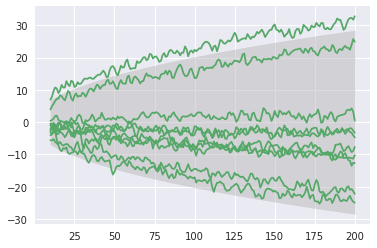
\includegraphics[width=\textwidth]{images/profile_kernel_prior}
        \caption{Prior distribution and some samples; the grey area is the 95\% confidence interval.}
        \label{fig:kernel_prior}
    \end{subfigure}
    \hfill
    \begin{subfigure}[t]{0.45\textwidth}
        \centering
        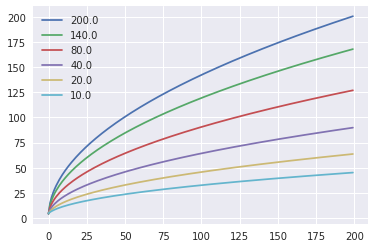
\includegraphics[width=\textwidth]{images/kernel_values}
        \caption{Values of the kernel: each line corresponds to a different value of $z_1$, and $z_2$ is on the ordinate.}
        \label{fig:kernel_values}
    \end{subfigure}
    \caption{Behavior of the kernel in equation \ref{eq:kernel}, where the altitude is on the $x$ axis, and the predicted value on the $y$ axis. Notice the approximate logarithmic profile with which the predicted value changes with altitude; this is caused by the square root term in the kernel, and emulates the effect of the $\ln z$ term in equation \ref{eq:logmodel}.}
	\label{fig:kernel}
\end{figure}

Our final goal is to obtain the derivative of the predictive posterior mean, which can be done using equation \ref{eq:gp_gradient}; for this we need to derive equation \ref{eq:kernel} with respect to $z_1$:

\begin{equation}
\label{eq:kernel_derivative}
\frac{\partial k(z_1,z_2)}{\partial z_1}=\frac{z_2-z_1}{\sigma_0^2}\exp\left(-\frac{(z_1-z_2)^2}{\sigma_0^2}\right)+\frac{z_2}{2\sqrt{\sigma_1^2+z_1z_2}}+\sigma_2^2\mathbbm{1}[z_1=z_2]
\end{equation}

\section{Monin-Obukhov Similarity Theory}
\label{sec:most_fit}

Even though there is agreement on form of their form, there is still debate on the exact values of the coefficients, with different experiments resulting in different values \citep{hogstrom88}. In order to ensure a fair comparison with the results of this work, we fit the universal functions to the data from the Cesar database. Their general form is:

\begin{equation}
\label{eq:phi_general}
\phi(\xi)=\begin{cases}
a+b\xi & \xi\geq 0 \\
a(1-c^2\xi)^d & \xi<0 \\
\end{cases}
\end{equation}

Where $a$ is close to 1, $b$ is positive, and $d$ is negative. Since $d$ is negative, the base of the power must be positive, hence the squared $c$. Following the approach outlined in section \ref{sec:regression_fit}, the coefficients $a$, $b$, $c$ and $d$ can be found by minimizing the L2-regularized mean squared error using equations \ref{eq:least_squares_gradient} and \ref{eq:least_squares_hessian}; in this case, the parameter vector is $\bm\theta=\left[a,b,c,d\right]^\intercal$. The gradient of \ref{eq:phi_general} is:


\begin{align}
\nabla_\theta\phi(\xi)\vert_{\xi\geq 0}=\begin{bmatrix}
1 \\ \xi \\ 0 \\ 0
\end{bmatrix} &&
\nabla_\theta\phi(\xi)\vert_{\xi<0}=\begin{bmatrix}
\tau^d \\ 0 \\ -2acd\xi\tau^{d-1} \\ a\tau^d\ln\tau
\end{bmatrix}
\end{align}

where $\tau=1-c^2\xi$. The Hessian of \ref{eq:phi_general} when $\xi\geq 0$ is simply 0, because it is a linear function in all parameters, while, in the negative case, we have:

\begin{equation}
\nabla^2_\theta\phi(\xi)\vert_{\xi<0} = \begin{bmatrix}
0 & 0 & - 2 c d \xi \tau^{d - 1} & \tau^{d} \ln{\tau} \\
0 & 0 & 0 & 0 \\
- 2 c d \xi \tau^{d - 1} &
0 & \frac{2ad\xi\tau^{d}}{c^4\xi^2+\tau}\left(2c^2d\xi-c^2\xi-1\right) & -2ac\xi\tau^{d-1}\left(d\ln\tau+1\right) \\
\tau^d \ln\tau & 0 &
-2ac\xi\tau^{d-1}\left(d\ln\tau+1\right) &
\tau^d\ln^2\tau
\end{bmatrix}
\end{equation}

Analytical computation of the Hessian allows us to use the Newton conjugate gradient descent algorithm, which provides super-linear convergence rate, unlike other conjugate gradient methods whose rate of convergence is only linear \citep{numopt}.

This model is then fitted to the data using L2 regularization, and evaluated as the other regression models; see section \ref{sec:perf_eval} for details on the procedure.

\section{Model Fitting}
\label{sec:model_fit}
In this section, we discuss how we use the data from the Cesar database to predict $\phi_m$.

\subsection{Features}
All the features come from the Cesar database, refer to section \ref{sec:data_collection} for details on how the data was collected. The predictors are partitioned in five sets:

\begin{enumerate}
\item[F1:] altitude $z$, wind at $z$, temperature at $z$, wind at 10 meters, temperature at 10 meters, wind at 20 meters, temperature at 20 meters, wind at 40 meters, temperature at 40 meters, soil temperature;
\item[F2:] Soil heat flux;
\item[F3:] Net radiation;
\item[F4:] Rain amount, dew point;
\item[F5:] Turbulent kinetic heat flux, turbulent latent heat flux;
\end{enumerate}

These sets are used cumulatively in the order they are listed, meaning that, for example, F3 is used in conjunction with F2 and F1. Derived features that can be computed from others, such as the virtual temperature (equation \ref{eq:vtemp}), are not included. The reason is that the less inputs the models require, the more useful and "agile" they can be when used as a component in a larger system, such as climate simulations.

This division was decided based on domain knowledge, so that the level of a feature reflects both its expected impact on the performance and how desirable it is to include it. An example of the former reasoning is with F4, where the effect of moisture is expected to be captured by the soil heat flux, and to be generally negligible in all but the most extreme conditions. An example of the latter reasoning is with F5, because turbulent fluxes are hard to measure accurately (see section \ref{sec:eddy_correlation}), and current simulation models are known to be quite inaccurate in their estimation of these fluxes \citep{sheba}. Similarly, the friction velocity was not included, because the point of predicting $\phi_m$ is to use it to estimate $u_*$ from the wind gradient, which is readily measured both in real life and in simulations. \cite{cabauw_z0} has shown that the direction of the wind affects the universal functions at Cabauw, because of the different covers of the surface, changing the roughness length, and disturbances by the main mast, preventing accurate wind speed measurement. Nonetheless, we decided not to include the wind direction in the features, as this is very specific to the Cabauw observatory, and would reduce the generality of our models.

We also create a second version of each feature set, augmented with the hourly trend of each variable, except for the altitude $z$. The reason for including the trend is that it can give an indication of, for example, the time of the day, or other complex phenomena for which there is no measurement. The interval for the trend (one hour) is used because it is enough to capture local variations, but not too large so as to contain irrelevant information. The hourly trend is computed simply as the difference between the current value and the value measured one hour before, divided by one hour. Given the goal of this work, namely to produce a model to be used in climate simulations, it would not make sense to use future values to compute the trend.

Finally, each feature is centered and standardized so as to have zero mean and unit standard deviation:

\begin{equation}
\label{eq:standardization}
x^\prime_{i,j}=\frac{x_{i,j}-\mu_j}{\sigma_j}
\end{equation}

This method is not robust to outliers, since they heavily affect mean and standard deviation; this can be prevented by subtracting the median and normalizing with the interquartile range instead. These two methods give similar results in our datasets, therefore we follow equation \ref{eq:standardization}, since it it the most widely used in practice. Obviously, every $\mu_j$ and $\sigma_j$ are computed only on the training data, and used to normalize both training and testing data.

\subsection{Models}

The models that we use are ridge regression, k-nearest neighbors, gradient boosted trees, and neural networks. Due to the size of the dataset, we cannot use kernel-based algorithms such as SVM and Gaussian Processes, as they require $\Theta(N^2)$ memory to store the kernel matrix, and $O(N^3)$ time to invert it. Gradient boosted trees were used instead of random forests because they were shown to work slightly better [citation], and small-scale experiments on our dataset showed they can be fit almost an order of magnitude more quickly.

All models but neural networks are fitted using nested cross validation with random hyper-parameter search. This procedure detailed in section \ref{sec:perf_eval}, but we list here the distributions of the hyper-parameters that we use in the random search:

\begin{itemize}
\item Ridge regression and Monin-Obukhov estimator: the only hyper-parameter to tune is the regularization coefficient, for which we use a log$_{10}$-uniform distribution\footnote{a random variable $X$ has a log$_\beta$-uniform distribution from $a$ to $b$ if $\log_\beta X$ is uniformly distributed between $a$ and $b$. Equivalently, if $Y$ is uniform between $a$ and $b$, then $\beta^Y$ is log$_\beta$-uniform.} from $10^{-6}$ to $10^{1}$.

\item k-nearest neighbors: the hyper-parameters to tune are the number of neighbors, chosen uniformly from $1$ to $15$, the distance function, either L1 or L2 norm, and the weights of the neighbors, either uniform or directly proportional to the distance to the query point.

\item Gradient boosted trees: the distributions are shown in table \ref{tbl:gb_hyperparams}. Note that $\delta$, for the Huber loss, refers to the percentile of the residuals, so that $\delta=0.5$ uses L2 loss for the smallest 50\% and L1 loss for the largest 50\%.
\end{itemize}

We use log-uniform distributions for parameters with a high range of possible values to reflect the intuition that small values are as likely as large values, and to avoid the samples being dominated by the larger values. Samples from an uniform distribution from $10^0$ to $10^3$ are ten times more likely to be from $[10^2,10^3]$ than from $[10^1,10^2]$, and, on average, only one in 100 samples will be in $[10^0,10^1]$. Log$_{10}$-uniform distributions do not have this problem, and a sample is equally likely to belong to any of the three intervals.

todo talk about nnets
 - use prelu instead of relu because relus get stuck
 - use dropout instead of batch norm + l2 regu because works better

\begin{table}[]
\centering
\caption{Distribution of the hyper-parameters for gradient boosted trees}
\label{tbl:gb_hyperparams}
\begin{tabularx}{\textwidth}{r|l|X}
\textbf{Hyper-parameter} & \textbf{Distribution} & \textbf{Values} \\ \hline
Number of estimators & log$_{10}$-uniform & From $10^1$ to $10^4$ \\
Learning rate & log$_{10}$-uniform & From $10^{-3}$ to $10^0$ \\
Number of features & Uniform & All possible values \\
Maximum depth & Uniform & From 4 to 12 \\
Sub-sampling factor & Uniform & From 25\% to 100\% \\
Loss function & Uniform & Least squares, least absolute deviation, \newline Huber loss (equation \ref{eq:huberloss}) \\
$\delta$ (for the Huber loss) & Uniform & From 1\% to 99\%
\end{tabularx}
\end{table}



\section{Performance Evaluation}
\label{sec:perf_eval}
The goal of performance evaluation is to obtain a realistic and unbiased estimate of the performance of a model on unseen data. Because the Monin-Obukhov similarity theory is only valid in the $-2\leq\xi\leq1$ range, we will use this data as the primary target for evaluation. We will also evaluate the models on the full dataset, to see what kind of performance can be expected outside of the typical range where the similarity theory is employed.

We are actually not interested in the optimal values of the hyper-parameters; for this reason, we perform nested cross validation, with the inner loop used to optimize the hyper-parameters through random search \citep{random_search}, and the outer loop used to evaluate the model. We use 10 folds in both the inner and outer CV, and test 10 different hyper-parameter combinations for all estimators. Limits in the available computational resources prevent us from testing more combinations; the possibility that this number is too low can manifest itself in the high variance of the nested cross validation results. Algorithm \ref{alg:nested_cv} shows in detail how nested cross validation with random search works.

In practice, we need to run $2\cdot5\cdot2=20$ nested cross validation rounds for each model, meaning that it is fit $20(10\cdot10\cdot10+10)=20200$ times in total. According to the model and its hyper-parameters, fitting can take from a few seconds up to more than 24 hours; in order to make the process feasible, we implemented algorithm \ref{alg:nested_cv} using Apache Spark \citep{spark}. Since the number of stragglers is very low\footnote{for gradient boosted trees, the slowest method, the median fitting time in our experiments is around half a minute, the third quartile is around ten minutes, and the maximum is between 20 and 30 hours}, running multiple nested cross validation jobs at the same time can reduce the duration of the whole process by five to ten times.

A fundamental assumption underlying hold-out evaluation methods is that the samples in the training set are independent and identically distributed, so that the distribution in the two partitions are equal. This is not our case, since there is a inherent time dependency in the data, meaning that samples obtained close in time are very similar. This can be confirmed by training and evaluating a k-nearest neighbors classifier with $k=1$ on random splits: the resulting mean squared error is in the order of $10^{-3}$, which is clearly unrealistic. To circumvent this problem, the CV folds are created on \emph{months}: all the samples in a given month and year are either in the training set or in the validation set. We choose months instead of days because the weather often does not change significantly in the span of 24 hours, whereas in a month there are around three weeks worth of samples that are independent from the conditions at the start and end of the month.

The main evaluation metric is the mean squared error, since that is what we are optimizing for, but we compute other metrics in the outer cross validation loop to get a more complete idea of the performance of the estimators:

\begin{itemize}
\item Mean Squared Error
\item Mean Absolute Error
\item Median Absolute Error
\item Mean Absolute Percent Error
\item Median Absolute Percent Error
\item $R^2$ Score:
$$
1-\frac{\sum (f_n-t_n)^2}{\sum (t_n-\overline{t})^2}
$$
\end{itemize}

Where $f_n$ is the predicted value for the test sample $\bm x_n$ with true value $t_n$, the squared error is $(f_n-t_n)^2$, the absolute error is $\vert f_n-t_n\vert$, the absolute percent error is $100\vert 1-f_n/t_n\vert$. We present both mean and median scores because the former are heavily skewed by outliers. We also present both absolute and percent errors because the latter are easier to interpret, but tend to explode when the true value is very small,\footnote{predicting 1 for a true value of 100 gives a percent error of 99\%, but predicting 100 for a true value of 1 gives, somewhat unfairly, a percent error of 9900\%} a condition that frequently happens in our dataset.

\begin{algorithm}
\caption{Nested cross validation with random hyper-parameter search.}
\label{alg:nested_cv}


\algnewcommand\algorithmicinput{\textbf{Input:}}
\algnewcommand\Input{\item[\algorithmicinput]}

\algnewcommand\algorithmicoutput{\textbf{Output:}}
\algnewcommand\Output{\item[\algorithmicoutput]}

\begin{algorithmic}
\Input \\
\begin{itemize}
\item[$D$] Dataset
\item[$K_O$] Number of outer folds
\item[$K_I$] Number of hidden folds
\item[$R$] Number of random combinations to try
\item[$model$] Model to train
\item[$distrs$] Distribution of each hyper-parameter
\end{itemize} \\
\Output Summary statistics computed on the outer validation fold \\

\For{$k_o\gets 1\ldots K_O$}\Comment{Outer $K_O$-fold cross validation}
	\State{Generate $k_o$-th outer fold $(D^o_T,D^o_V)$ from the dataset $D$}
	\State{$best\_mse\gets\inf$}
	\State{$best\_params\gets\bot$}
	\For{$r\gets 1\ldots R$}\Comment{Find best hyper-parameters on $D^o_T$}
		\State{$params\gets$ a random hyper-parameter combination from $distrs$}
		\State{$params\_mse\gets 0$}
		\For{$k_i\gets 1\ldots K_I$}\Comment{Evaluate $params$ with $K_I$-fold CV}
			\State{Generate $k_i$-th inner fold $(D^i_T,D^i_V)$ from $D^o_T$}
			\State{$model\gets$ a new instance of the model with parameters $params$}
			\State{Train $model$ on $D^i_T$}
			\State{$mse\gets$ result of the evaluation of $model$ on $D^i_V$}
			\State{$params\_mse\gets params\_mse+mse$}
		\EndFor

		\If{$params\_mse<best\_mse$}\Comment{MSE comparison on $K_i$-fold CV result}
			\State{$best\_mse\gets params\_mse$}
			\State{$best\_params\gets params$}
		\EndIf		
	\EndFor

	\State{$model\gets$ a new instance of the model with parameters $best\_params$}
	\State{Train $model$ on $D^o_T$}
	\State{Evaluate $model$ on $D^o_V$ and compute evaluation metrics}
\EndFor
\State{Compute summary of the metrics obtained in the outer loop}
\end{algorithmic}
\end{algorithm}

\section{Success Criteria}
\label{sec:success}
A successful answer to the first research question entails finding a model whose mean squared error on F5 with trend is smaller than the mean squared error of the Monin-Obukhov similarity theory estimator introduced in section \ref{sec:most_fit}.

The second research question is answered by comparing the different evaluation metrics on the ten feature sets (F1 to F5, with and without trend). Note that we cannot use the output of a model to obtain the importance of the features, as this method is not reliable when some of them are correlated \citep{rf_bias,rf_corr_imp}, which is a very relevant issue in our case. Trivially, wind speed and temperature at the different levels are very strongly correlated (Pearson's $r$ is above 0.95), and there are other, more complex, correlations, such as between the net radiation and the soil heat flux, or between the soil temperature and the dew point (Pearson's $r$ is respectively 0.75 and 0.79). In spite of the correlations, all these variables contribute to the flux-profile relationships, often in very nuanced ways.



\chapter{Results}
todo

\section{Exploratory Data Analysis}
The dataset consists of 17 years of measurements, from January 2001 to December 2017, for a total of 3 436 416 observations. Unfortunately, most of these observations contain low quality measurements, as detailed in section \ref{sec:data_filter}, leaving only  1 561 973 usable records. Additionally, the turbulent fluxes measured in March 2016 exhibit a much wider range than the March measurements of other years. Roughly 15 to 20\% of the measurements in that month are suspicious; since the Cesar database contains a separate dataset every month, we decided to completely exclude the dataset of March 2016, fearing for a systematic error somewhere in the process. Moreover, 6 measurements of the turbulent latent heat are way above the acceptable range, 4538 do not have a dew point , and 247 656 do not have a soil temperature. We do not attempt to impute missing values, because this process was already performed by the Cesar consortium, and we believe there is a good reason why these values were not imputed. This leaves 1 301 574 usable records.

Figure \ref{fig:le_season} shows the turbulent latent heat flux versus hour of day both in Winter and Summer, whereas figure \ref{fig:ustar_wind_temp} shows the friction velocity as a function of air temperature and wind speed. The dependency of $u_*$ with the wind speed of figure \ref{fig:ustar_wind} is quite complicated: there are three clear regions with different constant of proportionality and correlation coefficient. The group where the two quantities are almost perfectly correlated corresponds to imputed values for the friction velocity, derived from the wind speed. The three other groups differ widely in the values of the fluxes and radiation; for example, fitting an ordinary least squares model to 1000 bootstraps of the observations with negative net radiation yields an average proportionality coefficient of \num{0.051} with standard deviation \num{1.52e-05}, whereas the same procedure on the complementary set yields an average of \num{0.046} with standard deviation \num{1.40e-05}. Note that this dependency might be related to the observed imbalance in the surface energy budged, usually around 15\% during day time and 100\% during night time at the Cabauw observatory; \cite{cabauwinsitu} notes that the imbalance seems to depend on the speed of wind.

Talking about speed of wind, figure \ref{fig:ustar_wind} shows some measurements exceeding \SI{25}{\meter\per\second}; according to the Beaufort scale, holding umbrellas and walking become hard with wind at \SI{15}{\meter\per\second}. Those measurements are not issues with the data: figure \ref{fig:cyclone_jeanett} shows the highest wind speed present in the Cesar database to date, corresponding to cyclone Jeanett.

\begin{figure}
    \centering
    \begin{subfigure}[t]{0.48\textwidth}
        \centering
        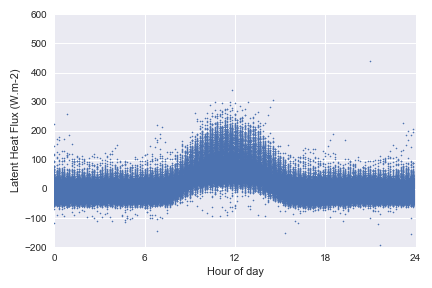
\includegraphics[width=\textwidth]{images/le_winter}
        \caption{Winter}
        \label{fig:le_winter}
    \end{subfigure}
    \hfill
    \begin{subfigure}[t]{0.48\textwidth}
        \centering
        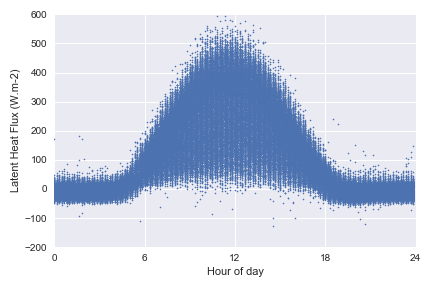
\includegraphics[width=\textwidth]{images/le_summer}
        \caption{Summer}
        \label{fig:le_summer}
    \end{subfigure}
    \caption{Turbulent latent heat flux versus hour of day in Winter (left) and Summer (right). One can see both the difference in day duration, and the effect of increased temperature on evaporation. The sensible heat flux follows a very similar pattern, with lower absolute values.}
	\label{fig:le_season}
\end{figure}


\begin{figure}
    \centering
    \begin{subfigure}[t]{0.48\textwidth}
        \centering
        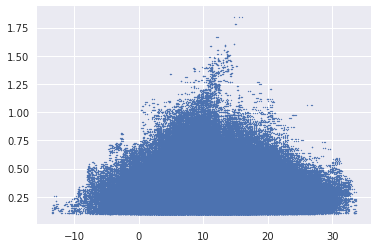
\includegraphics[width=\textwidth]{images/ustar_temp}
        \caption{Temperature}
        \label{fig:ustar_temp}
    \end{subfigure}
    \hfill
    \begin{subfigure}[t]{0.48\textwidth}
        \centering
        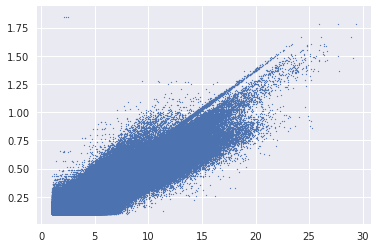
\includegraphics[width=\textwidth]{images/ustar_wind}
        \caption{Wind}
        \label{fig:ustar_wind}
    \end{subfigure}
    \caption{Friction velocity versus temperature (left) and wind speed (right). There is a clear subgroup where the wind and $u^*$ are almost perfectly correlated; this is because of the gap-filling technique discussed in section \ref{sec:gap_filling}. Additionally, there are three subgroups with different constant of proportionality; they differ widely in fluxes and radiation.}
	\label{fig:ustar_wind_temp}
\end{figure}

\begin{figure}
    \centering
	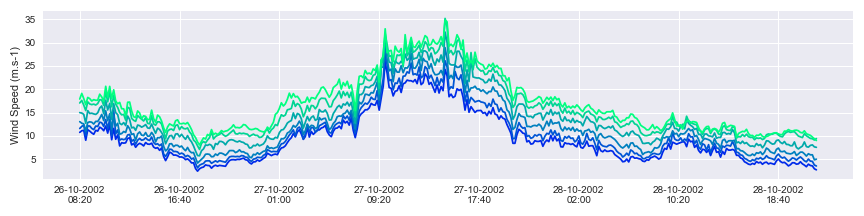
\includegraphics[width=0.95\textwidth]{images/cyclone_jeanett}
	\caption{Wind speed measurements during Cyclone Jeanett, which struck north-west Europe in October 2002, causing 33 fatalities. Although \SI{30}{\meter\per\second} wind is, in absolute terms, destructive, this cyclone registered winds up to \SI{42.5}{\meter\per\second}!}
	\label{fig:cyclone_jeanett}
\end{figure}



\section{Gradient Computation}
Section \ref{sec:gradients} introduced three different ways to compute the gradient, but we need to choose one to compute the universal functions. In this section, we refer to equation \ref{eq:fd_gradient} as \emph{F.D.}, equation \ref{eq:log_gradient} as \emph{Log} and equation \ref{eq:gp_gradient} as \emph{G.P.} Table \ref{tbl:gradients_corr} shows the Pearson correlation coefficient between the three methods, separately for every altitude level. It is clear that the F.D. gradient is inadequate at the lowest level; this can be explained by considering that equation \ref{eq:fd_gradient} with $z=10$ reduces to the wind speed at 20 meters divided by 20. This method appears to be too naive, especially since it does not take the roughness length into consideration, but, as \cite{cabauw_z0} showed, finding a value for $z_0$ is far from trivial. In spite of this, the F.D. and the Log gradients strongly agree on all levels, and are quite different from the gradients by G.P.

\begin{table}[]
\centering
\caption{Pearson correlation coefficient between the gradients predicted by the different methods, divided by level. The F.D. gradient is poorly correlated with the other two methods at the 10 meters level, but is very well correlated with the Log gradient at the other levels. The Log and G.P. gradients disagree on the lower levels, but it appears their predictions converge as altitude increases.}
\label{tbl:gradients_corr}
\begin{tabular}{c|c|c|c}
z & F.D. / G.P. & Log / F.D. & Log / G.P. \\ \hline
 	10 & 	0.192 & 0.480 &	0.317 \\
 	20 &	0.645 	& 0.991 &	0.640 \\
 	40 &	0.863 & 0.981 &	0.835 \\
\end{tabular}
\end{table}

Since Log and G.P. predict the wind speed too, we can compare their predictions to the measured wind speed. Notice that these methods are fitted on the wind speed at all levels, from 10 to 200 meters, but we evaluate them only on the three lowest levels, since that is where we compute the universal functions. Table \ref{tbl:model_wind_errors} shows the squared error between the modeled wind and the true wind speed at the three levels for both models. It is interesting to see that both models are quite accurate at all levels; this allows us to conclude that F.D. is not reliable at 10 meters.

\begin{table}[]
\centering
\caption{Absolute percent error of the wind speed modeled by the Log and G.P. methods at each altitude level. The altitude does not affect the error, and the G.P. wind speed is closer to the true wind speed than the Log model in the vast majority of cases, although the difference is negligible, often less than a few percents.}
\label{tbl:model_wind_errors}
\begin{tabular}{c|ccc|ccc|ccc}
& z & Log & G.P. & z & Log & G.P. & z & Log & G.P. \\\hline
mean & \multirow{7}{*}{ 10 } & 1.2250 & 1.0329 & \multirow{7}{*}{ 20 } & 2.2605 & 1.4217 & \multirow{7}{*}{ 40 } & 1.3878 & 1.0364 \\
std & & 1.4033 & 1.1169 & & 2.3432 & 1.4658 & & 1.4783 & 1.1208 \\
min & & 0.0000 & 0.0000 & & 0.0000 & 0.0000 & & 0.0000 & 0.0000 \\
25\% & & 0.3714 & 0.3249 & & 0.7447 & 0.4549 & & 0.4744 & 0.3037 \\
50\% & & 0.8217 & 0.7608 & & 1.6251 & 1.0595 & & 1.0263 & 0.7265 \\
75\% & & 1.5505 & 1.4179 & & 2.9642 & 1.9693 & & 1.8413 & 1.4143 \\
max & & 53.7541 & 212.3985 & & 106.5623 & 192.9434 & & 80.3531 & 43.4657 \\
\end{tabular} 
\end{table}


Figure \ref{fig:gp_log_perc_err_wind_speed} shows the error as a function of the wind speed. It is interesting to see that G.P. becomes more and more reliable as the wind speed increases; not only does its error decrease, so does the variance of the error. It is possible to give an intuitive explanation for the error of Log: the measurement error of the wind speed is the maximum between \SI{0.1}{\meter\per\second} and 1\%, therefore the error of Log can be attributed almost entirely to uncertainty in the data, whereas G.P. is, possibly, overfitting.

\begin{figure}
    \centering
	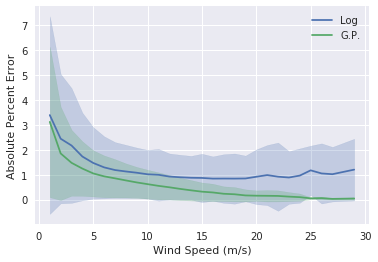
\includegraphics[width=0.75\textwidth]{images/gp_log_perc_err_wind_speed}
	\caption{Mean absolute percent error of the wind modeled by the Log and G.P. models as a function of the true wind speed; the lines are the average, and the shaded regions enclose the average plus or minus the standard deviation. Both quantities are computed by binning the wind by its integral part. Notice that only wind 656 observations, or 0.04\% of the total, are above \SI{20}{\meter\per\second} (\SI{72}{\kilo\meter\per\hour}), and slightly less than 5\% are above \SI{11}{\meter\per\second}.}
	\label{fig:gp_log_perc_err_wind_speed}
\end{figure}


Given that the final goal of finding the gradient is to compute the universal functions, for which we already have more or less agreed upon expressions (equation \ref{eq:phi_m_coeff}), it makes sense to compare the error of these expressions when predicting the universal functions (equation \ref{eq:phi_m}) computed with the gradients coming from the three different methods; the best method is, then, the one with the smallest error. Table \ref{tbl:gradient_errors} contains these errors, and shows that Log is the undisputed winner. Not considering the 10 meters level, F.D. is as good as Log, consistently with their very high correlation shown in table \ref{tbl:gradients_corr}.


\begin{table}[]
\centering
\caption{Mean squared error of $\phi_m$ (coefficients according to equation \ref{eq:phi_m_coeff}) when predicting the empirical flux-profile relationship (equation \ref{eq:phi_m}), computed with the three methods of calculating the gradient. The errors in second line (F.D. w/o z=10) were computed after discarding the data at the 10 meters level, because we argued the F.D. method is not reliable at that level. We show the error both in the range where the Monin-Obukhov similarity theory is known to be valid (84\% of the total), and the error using all data.}
\label{tbl:gradient_errors}
\begin{tabular}{r|c|c}
Method & MSE ($-2\leq\xi\leq1$) & MSE \\ \hline
F.D. & 1.994 & 9.322 \\
F.D. (w/o z=10) & 0.627  & 11.832 \\
Log & 0.660 & 8.498 \\
G.P. & 1.213 & 8.899
\end{tabular}
\end{table}

To conclude, although F.D. (equation \ref{eq:fd_gradient}) is the most accurate way of computing the profile gradient, it does not allow us to use data at the 10 meters level. Considering that Log (equation \ref{eq:log_gradient}) is very slightly worse, but allows us to include that level (increasing the data available by 50\%!), all the results presented from now on make use of it.


\section{Flux-Profile Relationship}
Figure \ref{fig:most_scatter} shows the wind shear versus the instability parameter, together with the commonly accepted flux-profile relationship and the relationship fitted on our dataset, and in figure \ref{fig:most_zoom} we see the flux-profile relationship restricted to the interval of instability parameter where the Monin-Obukhov similarity theory is valid. Qualitatively, the relationship behaves as expected, going to zero as $\xi$ decreases, linearly increasing in the $0\leq\xi\leq1$ interval, and leveling after that. Refer to section \ref{sec:most_estimator_results} for further details.

negative phim with small |xi|


\begin{figure}
    \centering
    \begin{subfigure}[t]{0.48\textwidth}
        \centering
        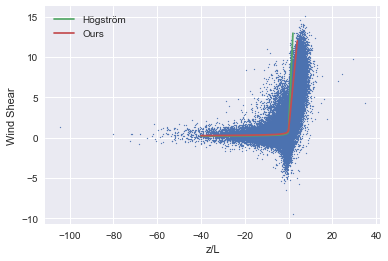
\includegraphics[width=\textwidth]{images/most_full}
        \caption{Full dataset}
        \label{fig:most_full}
    \end{subfigure}
    \hfill
    \begin{subfigure}[t]{0.48\textwidth}
        \centering
        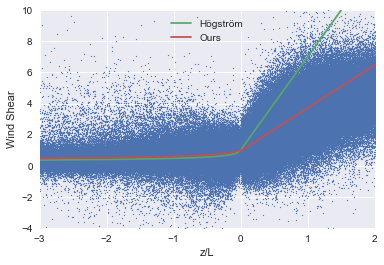
\includegraphics[width=\textwidth]{images/most_zoom}
        \caption{Validity region for the Monin-Obukhov similarity theor.}
        \label{fig:most_zoom}
    \end{subfigure}
    \caption{Wind shear $\phi_m$ versus the instability parameter $\xi$, with the prediction according to equation \ref{eq:phi_m_coeff} in green, and our predictions, following equation \ref{eq:phi_general} with the coefficients being the median values in table \ref{tbl:most_coeffs}, in red.}
	\label{fig:most_scatter}
\end{figure}


\section{Model Comparison}
performance of the models


\subsection{MOST Estimator}
\label{sec:most_estimator_results}
The performance of the MOST estimator is shown in table \ref{tbl:most_results}; the proportion of data for which $-2\leq\xi\leq 1$ is 83.6\%. We see a considerable increase in the MSE when the full dataset is used; this is not surprising, considering that, with $\xi>1$, $\phi_m$ tends to level off, and there are a considerable number of outliers in the range $-20\leq\xi\leq-2$ (see figure \ref{fig:most_full}) that cannot be fitted by the MOST estimator. Figure \ref{fig:most_scatter} shows $\phi_m$ as a function of $\xi$ as computed in our dataset, as well as the predictions of equation \ref{eq:phi_m_coeff} and the fitted MOST estimator.

Table \ref{tbl:most_results} shows the values of the coefficients in equation \ref{eq:phi_general}, when fitted to the region of data where the Monin-Obukhov similarity theory is valid. We note a big difference with the values recommended in \cite{hogstrom88}, as well as most studies on the topic. However, \cite{cabauw_night_most} studied the stable, nocturnal boundary layer at Cabauw, and reported values varying between 0.81 and 0.95 for $a$ and between 2.7 and 3.2 for $b$, depending on the direction of the wind; there is no known explanation for this discrepancy. Although these values were obtained with linear regression, essentially the same method that we applied, no goodness of fit statistics, such as MSE or $R^2$, were reported.

\begin{table}[]
\centering
\caption{Evaluation metrics for the Monin-Obukhov estimator}
\label{tbl:most_results}
\begin{tabular}{r|c|c|c|c}
& \multicolumn{2}{c|}{All} & \multicolumn{2}{c}{$-2\le\xi\le1$} \\
 & Mean & Std.  & Mean & Std. \\ \hline
Mean Squared Error 					& 0.672028  		& 0.031320  & 0.332056    & 0.017246     \\
$R^2$ Score									& 0.705471    	& 0.008943 & 0.605013    & 0.010732       \\
Mean Absolute Error 					& 0.540632  		& 0.013878 & 0.395410    & 0.007181      \\
Median Absolute Error 				& 0.371569 		& 0.015601 & 0.282736    & 0.004304      \\
Mean Absolute Percent Error  	& 252.925389 	& 196.086056 & 184.707665   & 48.260311    \\
Median Absolute Percent Error	& 28.964847  	& 0.938811 & 24.618438    & 0.729602   
\end{tabular}
\end{table}

\begin{table}[]
\centering
\caption{Values of the coefficients of the MOST estimator of equation \ref{eq:phi_general} fitted on the data with $-2\leq\xi\leq1$. The minimum values for $c$ and $d$ seem to be outliers, as well as the next smallest value, but the other 8 values are closely clustered together within an interval of about 0.15.}
\label{tbl:most_coeffs}
\begin{tabular}{r|c|c|c|c|c|c|c}
   & Mean       & Std.       & Min.       & 25\%       & 50\%       & 75\%       & Max. \\ \hline
$a$   & 0.943802  & 0.004228  & 0.935826  & 0.942926  & 0.944624  & 0.946017  & 0.950583 \\
$b$   & 2.772180  & 0.008216  & 2.758320  & 2.769266  & 2.772188  & 2.778464  & 2.783730 \\
$c$   & 2.452160  & 0.469983  & 1.246522  & 2.607285  & 2.646705  & 2.674603  & 2.713834 \\
$d$   & -0.298687  & 0.109407 & -0.601655 & -0.261012 & -0.258147 & -0.255400 & -0.248226
\end{tabular}
\end{table}


\subsection{Ridge Regression}

\begin{figure}
\centering
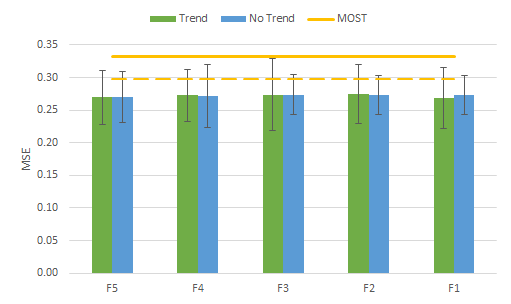
\includegraphics[width=\textwidth]{images/ridge_results}
\caption{Performance of the Ridge regression estimator on the five feature sets with and without trend; the error bars are two standard deviations long in each direction. The solid yellow line is the performance attained by the MOST estimator, and the dashed yellow is that minus two standard deviations.}
\label{fig:ridge_results}
\end{figure}

\begin{table}[]
\centering
\caption{Evaluation metrics for the Ridge linear regression estimator on the five feature sets augmented with trend.}
\begin{tabular}{c|r|c|c|c|c}
& & \multicolumn{2}{c|}{All} & \multicolumn{2}{c}{$-2\le\xi\le1$} \\
&  & Mean & Std. & Mean & Std.   \\ \hline
 \multirow{6}{*}{F5} & Mean Squared Error 					& 0.593038  		& 0.048443  & 0.168731    & 0.016571    \\
& $R^2$ Score									& 0.734663     	& 0.017526 & 0.688497    & 0.029011      \\
& Mean Absolute Error 					& 0.509204  		& 0.018504 & 0.284076    & 0.011686      \\
& Median Absolute Error 				& 0.345660 		& 0.009037   & 0.204298    & 0.005318    \\
& Mean Absolute Percent Error  	& 264.613746 	& 298.463690 & 79.669309   & 30.583787   \\
& Median Absolute Percent Error	& 27.816959  	& 1.286721  & 19.301579    & 0.565164  \\ \hline
 \multirow{6}{*}{F4} & Mean Squared Error 					& a & b & 0.168744   & 0.012348   \\
& $R^2$ Score									& a & b & 0.689096   & 0.018279   \\
& Mean Absolute Error 					& a & b & 0.284449   & 0.010863   \\
& Median Absolute Error 				& a & b & 0.205146    & 0.006771   \\
& Mean Absolute Percent Error  	& a & b & 80.805403  & 34.558653  \\
& Median Absolute Percent Error	& a & b & 19.327348   & 0.538968  
\end{tabular}
\end{table}



\begin{table}[]
\centering
\caption{Evaluation metrics for the k-nearest neighbors estimator on the five feature sets augmented with trend.}
\label{tbl:knn_results_f5t}
\begin{tabular}{c|r|c|c|c|c}
& & \multicolumn{2}{c|}{All} & \multicolumn{2}{c}{$-2\le\xi\le1$} \\
& & Mean & Std. & Mean & Std.   \\ \hline
\multirow{6}{*}{F5} & Mean Squared Error 					& 0.583102   	& 0.035314  & 0.187911    & 0.009168    \\ 
& $R^2$ Score									& 0.739219   	& 0.010517 & 0.653668    & 0.009450      \\
& Mean Absolute Error 					& 0.487180   	& 0.016797  & 0.314231    & 0.006526     \\
& Median Absolute Error 				& 0.300725   	& 0.011178  & 0.237316    & 0.005357       \\
& Mean Absolute Percent Error  	& 151.571688	&  55.287673 & 98.785002   & 39.723715    \\
& Median Absolute Percent Error	& 25.450125   	& 1.270630  & 21.959704    & 0.538930 \\ \hline
\multirow{6}{*}{F4} & Mean Squared Error 					& a & b & 0.197570   & 0.006350   \\ 
& $R^2$ Score									& a & b & 0.635371   & 0.010965   \\
& Mean Absolute Error 					& a & b & 0.321321   & 0.005622   \\
& Median Absolute Error 				& a & b & 0.241515   & 0.004917   \\
& Mean Absolute Percent Error  	& a & b & 98.139450  & 40.602436  \\
& Median Absolute Percent Error	& a & b & 22.339853    & 0.829702  \\ \hline
\end{tabular}
\end{table}


\begin{table}[]
\centering
\caption{Evaluation metrics for the gradient boosting estimator on the five feature sets augmented with trend.}
\label{tbl:gb_results_f5t}
\begin{tabular}{c|r|c|c|c|c}
& & \multicolumn{2}{c|}{All} & \multicolumn{2}{c}{$-2\le\xi\le1$} \\
\multirow{6}{*}{F5} & Mean & Std. & Mean & Std.   \\ \hline
& Mean Squared Error 					& 0.285956	& 0.012074 & 0.087484    & 0.007147    \\  
& $R^2$ Score									& 0.872323   & 0.006331   & 0.838710    & 0.008769    \\
& Mean Absolute Error 					& 0.319557   & 0.006457 & 0.192329    & 0.007915    \\
& Median Absolute Error 				& 0.180583  	& 0.003956   & 0.127258    & 0.006362   \\
& Mean Absolute Percent Error		& 88.093397	& 53.138612  & 43.165082   & 13.711617   \\
& Median Absolute Percent Error	& 15.888091	& 0.499692 & 12.523625    & 0.535662   \\ \hline
\multirow{6}{*}{F4} & Mean Squared Error 					& a & b & 0.093117   & 0.006277   \\ 
& $R^2$ Score									& a & b & 0.828070   & 0.006365   \\
& Mean Absolute Error 					& a & b & 0.201683      & 0.007324   \\
& Median Absolute Error 				& a & b & 0.136112   & 0.006557   \\
& Mean Absolute Percent Error  	& a & b & 45.666477  & 10.974657  \\
& Median Absolute Percent Error	& a & b & 13.447042   & 0.706335  \\ \hline
\end{tabular}
\end{table}




\chapter{Discussion}
even though we predicted phim, the actual interest is in u*. we predict phim to have a direct means of comparing with state of the art

actual constants and coefficients (e.g. von karmans constant) dont really matter, because they are constant and do not affect the ml model 

estimating parameters (von karman, roughness length etc) is very difficult, by using ml we can circumvent the problem (they need a supporting infrastructure even if they want to compute those constants, so not huge downside)

outliers with xi between -20 and -2 mostly belong to z=40 in the morning (between 6 and 12); given what was said in [paper], there is the possibility that they are not in the surface layer, explaining why the c coefficient is higher than expected

one of the reasons why MOST is unreliable in stable conditions is because of the difficulty of measuring fluxes. there are other methods to compute the turbulent fluxes (http://bibliotheek.knmi.nl/knmipubWR/WR87-02.pdf, ), we used eddy corr because that's what in the cesar database

our models can only be used in conditions that are similar to cabauw. most importantly, they are not valid in the oceanic surface layer, because it is very different [citation]

\section{Limitations and Future Work}
todo


%\bibliographystyle{unsrt}
%\bibliographystyle{plainnat}
\bibliographystyle{agsm}
\bibliography{thesis}

\end{document}
